\documentclass[12pt,a4paper]{article}

% ── Packages ──
\usepackage[margin=1in]{geometry}
\usepackage{amsmath,amssymb}
\usepackage{graphicx}
\usepackage{booktabs}
\usepackage{array}
\usepackage{multirow}
\usepackage{enumitem}
\usepackage{xcolor}
\usepackage{tcolorbox}
\usepackage{tikz}
\usepackage{fancyhdr}
\usepackage{hyperref}
\usepackage{float}
\usepackage{caption}
\usepackage{longtable}
\usepackage{tabularx}

\usetikzlibrary{automata, positioning, arrows.meta, calc, shapes.geometric}

% ── Colors ──
\definecolor{primary}{RGB}{0,73,144}
\definecolor{accent}{RGB}{220,50,50}
\definecolor{successgreen}{RGB}{34,139,34}
\definecolor{warncolor}{RGB}{200,120,0}
\definecolor{lightbg}{RGB}{240,245,255}
\definecolor{errorbg}{RGB}{255,235,235}
\definecolor{tipbg}{RGB}{235,255,235}
\definecolor{gold}{RGB}{255,200,0}

% ── tcolorbox styles ──
\tcbuselibrary{breakable,skins}

\newtcolorbox{importantbox}[1][]{
  colback=errorbg, colframe=accent, fonttitle=\bfseries,
  title={#1}, breakable, sharp corners, boxrule=1pt
}

\newtcolorbox{tipbox}[1][]{
  colback=tipbg, colframe=successgreen, fonttitle=\bfseries,
  title={#1}, breakable, sharp corners, boxrule=1pt
}

\newtcolorbox{infobox}[1][]{
  colback=lightbg, colframe=primary, fonttitle=\bfseries,
  title={#1}, breakable, sharp corners, boxrule=1pt
}

% ── TikZ styles ──
\tikzset{
  state/.style={
    circle, draw=primary, thick, minimum size=1.2cm,
    inner sep=2pt, font=\footnotesize\bfseries, fill=lightbg
  },
  every edge/.style={draw, ->, >=Stealth, thick, font=\footnotesize},
  accept/.style={state, double, double distance=2pt},
  reset/.style={draw=none, fill=none, minimum size=0},
  mealy output/.style={font=\footnotesize\color{accent}},
}

% ── Header / Footer ──
\pagestyle{fancy}
\fancyhf{}
\fancyhead[L]{\textcolor{primary}{\textbf{FSM Design Guide}}}
\fancyhead[R]{\textcolor{primary}{Digital System Design}}
\fancyfoot[C]{\thepage}
\renewcommand{\headrulewidth}{0.5pt}

\hypersetup{
  colorlinks=true, linkcolor=primary, urlcolor=primary
}

% ══════════════════════════════════════════════════════════════════
\begin{document}

% ── Title Page ──
\begin{titlepage}
\centering
\vspace*{2cm}
{\Huge\bfseries\textcolor{primary}{Finite State Machine\\Design Guide}\par}
\vspace{0.5cm}
{\Large\textcolor{accent}{From Fundamentals to Advanced\\Real-World Digital Systems}\par}
\vspace{2cm}

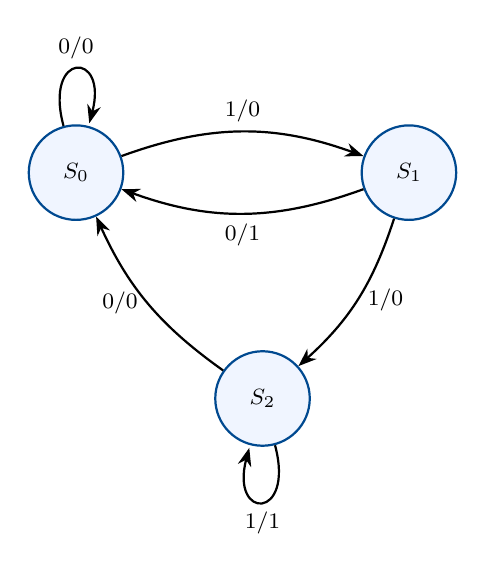
\begin{tikzpicture}[node distance=3cm]
  \node[state] (S0) {$S_0$};
  \node[state, right=of S0] (S1) {$S_1$};
  \node[state, below right=2cm and 1.5cm of S0] (S2) {$S_2$};
  \path (S0) edge[bend left=20] node[above]{1/0} (S1)
        (S1) edge[bend left=20] node[below]{0/1} (S0)
        (S1) edge[bend left=15] node[right]{1/0} (S2)
        (S2) edge[bend left=15] node[left]{0/0} (S0)
        (S0) edge[loop above] node{0/0} ()
        (S2) edge[loop below] node{1/1} ();
\end{tikzpicture}

\vspace{2cm}
{\large Digital System Design --- Advanced Level\par}
\vspace{0.5cm}
{\large\today\par}
\end{titlepage}

\tableofcontents
\newpage

% ══════════════════════════════════════════════════════════════════
\section{Introduction to Finite State Machines}
% ══════════════════════════════════════════════════════════════════

A \textbf{Finite State Machine (FSM)} is a mathematical model of computation consisting of:
\begin{itemize}
  \item A finite set of \textbf{states} $S = \{S_0, S_1, \ldots, S_{n-1}\}$
  \item A finite \textbf{input alphabet} $\Sigma$
  \item A \textbf{transition function} $\delta: S \times \Sigma \to S$
  \item An \textbf{output function} (Moore or Mealy)
  \item An \textbf{initial state} $S_0$
\end{itemize}

\subsection{Moore vs.\ Mealy Machines}

\begin{infobox}[Moore Machine]
Output depends \textbf{only} on the current state.\\
$\lambda: S \to \Gamma$ \quad (output function)\\
\textit{Outputs change synchronously with state transitions.}
\end{infobox}

\begin{infobox}[Mealy Machine]
Output depends on \textbf{both} the current state \textbf{and} input.\\
$\lambda: S \times \Sigma \to \Gamma$ \quad (output function)\\
\textit{Outputs can change asynchronously with input changes.}
\end{infobox}

\begin{figure}[H]
\centering
\begin{minipage}{0.45\textwidth}
\centering
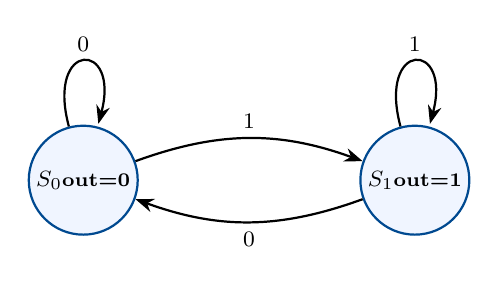
\begin{tikzpicture}[node distance=2.8cm]
  \node[state] (A) {$S_0$\\{\scriptsize out=0}};
  \node[state, right=of A] (B) {$S_1$\\{\scriptsize out=1}};
  \path (A) edge[bend left=20] node[above]{1} (B)
        (B) edge[bend left=20] node[below]{0} (A)
        (A) edge[loop above] node{0} ()
        (B) edge[loop above] node{1} ();
\end{tikzpicture}
\caption*{Moore Machine: output in state}
\end{minipage}
\hfill
\begin{minipage}{0.45\textwidth}
\centering
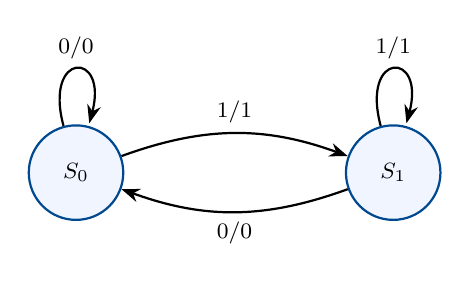
\begin{tikzpicture}[node distance=2.8cm]
  \node[state] (A) {$S_0$};
  \node[state, right=of A] (B) {$S_1$};
  \path (A) edge[bend left=20] node[above]{1/1} (B)
        (B) edge[bend left=20] node[below]{0/0} (A)
        (A) edge[loop above] node{0/0} ()
        (B) edge[loop above] node{1/1} ();
\end{tikzpicture}
\caption*{Mealy Machine: input/output on edges}
\end{minipage}
\end{figure}

\subsection{General FSM Architecture}

\begin{figure}[H]
\centering
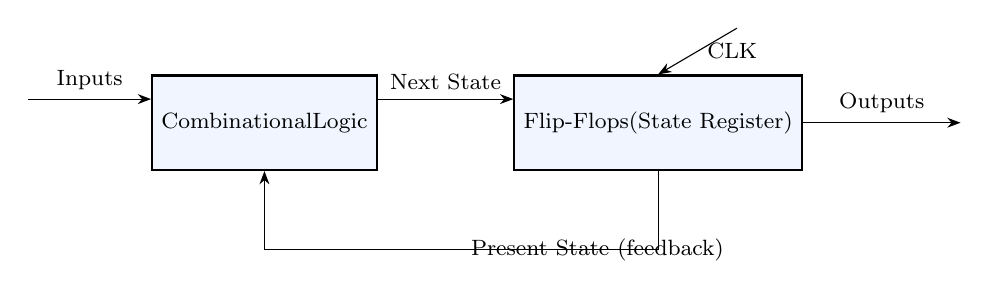
\begin{tikzpicture}[
  block/.style={draw, thick, minimum width=2.5cm, minimum height=1.2cm, fill=lightbg, font=\footnotesize},
  >=Stealth
]
  \node[block] (CL) at (0,0) {Combinational\\Logic};
  \node[block] (FF) at (5,0) {Flip-Flops\\(State Register)};
  \draw[->] (-3,0.3) -- (CL.west |- 0,0.3) node[midway, above]{\footnotesize Inputs};
  \draw[->] (CL.east |- 0,0.3) -- (FF.west |- 0,0.3) node[midway, above]{\footnotesize Next State};
  \draw[->] (FF.east) -- ++(2,0) node[midway, above]{\footnotesize Outputs};
  \draw[->] (FF.south) -- ++(0,-1) -| (CL.south) node[near start, right]{\footnotesize Present State (feedback)};
  \draw[->] (6,1.2) -- (FF.north) node[midway, right]{\footnotesize CLK};
\end{tikzpicture}
\caption{General FSM Block Diagram}
\end{figure}


% ══════════════════════════════════════════════════════════════════
\section{FSM Design Methodology --- Step by Step}
% ══════════════════════════════════════════════════════════════════

\begin{tipbox}[The Golden 8-Step Process]
\begin{enumerate}[leftmargin=*]
  \item \textbf{Understand the problem} --- identify inputs, outputs, and behaviour.
  \item \textbf{Draw the state diagram} --- all states, transitions, outputs.
  \item \textbf{Minimize states} --- merge equivalent states (implication chart).
  \item \textbf{Assign state encoding} --- binary, Gray, one-hot.
  \item \textbf{Build the state/transition table} --- present state, input, next state, output.
  \item \textbf{Derive the excitation table} --- using D flip-flop characteristics.
  \item \textbf{Obtain Boolean equations} --- K-maps for each flip-flop input and output.
  \item \textbf{Draw the circuit} --- connect flip-flops, gates, and I/O.
\end{enumerate}
\end{tipbox}

\subsection{D Flip-Flop Characteristic and Excitation}

The D flip-flop is the simplest memory element for FSM implementation.

\begin{table}[H]
\centering
\caption{D Flip-Flop Characteristic Table}
\begin{tabular}{cc|c}
\toprule
$D$ & CLK$\uparrow$ & $Q^+$ (Next State) \\
\midrule
0 & $\uparrow$ & 0 \\
1 & $\uparrow$ & 1 \\
\bottomrule
\end{tabular}
\end{table}

\begin{table}[H]
\centering
\caption{D Flip-Flop Excitation Table}
\begin{tabular}{cc|c}
\toprule
$Q$ (Present) & $Q^+$ (Next) & $D$ (Required Input) \\
\midrule
0 & 0 & 0 \\
0 & 1 & 1 \\
1 & 0 & 0 \\
1 & 1 & 1 \\
\bottomrule
\end{tabular}
\end{table}

\begin{infobox}[Key Insight]
For a D flip-flop: $D = Q^+$. The required D input is simply equal to the desired next state. This makes D flip-flops the easiest to use in FSM design!
\end{infobox}


\subsection{State Encoding Techniques}

\begin{table}[H]
\centering
\caption{Comparison of State Encoding Methods}
\begin{tabular}{lp{3cm}p{3cm}p{3cm}}
\toprule
\textbf{Encoding} & \textbf{Flip-Flops} & \textbf{Pros} & \textbf{Cons} \\
\midrule
Binary & $\lceil\log_2 n\rceil$ & Fewest flip-flops & Complex next-state logic \\
Gray Code & $\lceil\log_2 n\rceil$ & 1-bit change per transition & Limited applicability \\
One-Hot & $n$ & Simplest logic, fast & Many flip-flops \\
\bottomrule
\end{tabular}
\end{table}


% ══════════════════════════════════════════════════════════════════
\section{Common Errors in FSM Design}
% ══════════════════════════════════════════════════════════════════

\begin{importantbox}[Critical Mistakes to Avoid]
\begin{enumerate}[leftmargin=*]
  \item \textbf{Missing transitions:} Every state must have a defined transition for \emph{every} possible input combination. Missing transitions lead to undefined/stuck states.

  \item \textbf{Missing reset state:} Every FSM \emph{must} have a defined initial/reset state. Without it, the FSM powers up in an unknown state.

  \item \textbf{Unreachable states:} States that cannot be reached from the initial state waste resources and may cause problems if entered accidentally.

  \item \textbf{Dead-end states (latch-up):} States with no outgoing transitions trap the FSM forever.

  \item \textbf{Wrong state encoding:} Incorrect binary assignment leads to wrong excitation equations and faulty operation.

  \item \textbf{Glitches in Mealy outputs:} Since Mealy outputs depend on inputs, asynchronous input changes can cause output glitches.

  \item \textbf{Incorrect excitation table:} Confusing characteristic table with excitation table, or using JK/T excitation for D flip-flops.

  \item \textbf{Don't-care mishandling:} Unused states should be assigned don't-care or safe transitions, not left floating.

  \item \textbf{Clock domain issues:} Inputs not synchronized to the clock domain cause metastability.

  \item \textbf{State minimization errors:} Merging non-equivalent states changes the FSM's behaviour.

  \item \textbf{Output equation errors:} Computing output from next state instead of present state (Moore), or forgetting input dependency (Mealy).

  \item \textbf{Forgetting to handle unused states in implementation:} In a 3-flip-flop design with 5 used states, the 3 unused states (binary combinations) must transition to a safe state.
\end{enumerate}
\end{importantbox}


% ══════════════════════════════════════════════════════════════════
\section{Best Practices for FSM Design}
% ══════════════════════════════════════════════════════════════════

\begin{tipbox}[Professional Design Guidelines]
\begin{enumerate}[leftmargin=*]
  \item \textbf{Always start with a clear specification} --- list all inputs, outputs, and describe every scenario before drawing anything.

  \item \textbf{Draw the state diagram first} --- visual representation catches errors early.

  \item \textbf{Label everything} --- states, transitions (input/output), and reset arrows.

  \item \textbf{Check completeness} --- verify every state has transitions for all input combinations.

  \item \textbf{Handle unused states explicitly} --- assign them transitions to the reset state.

  \item \textbf{Use D flip-flops unless there's a specific reason not to} --- $D = Q^+$ simplifies everything.

  \item \textbf{Verify with a timing diagram} --- trace signals through time to validate.

  \item \textbf{Use simulation before hardware} --- ModelSim, Vivado, etc.

  \item \textbf{Prefer Moore when possible} --- glitch-free synchronous outputs.

  \item \textbf{Document your encoding} --- always write down which binary code maps to which state.
\end{enumerate}
\end{tipbox}


% ══════════════════════════════════════════════════════════════════
\section{From State Diagram to D Flip-Flop Implementation}
\label{sec:methodology}
% ══════════════════════════════════════════════════════════════════

This section walks through the \textbf{complete methodology} using a detailed example.

\subsection{Example: Sequence Detector (detects ``101'')}

\textbf{Specification:} Design a Moore FSM that outputs 1 when the sequence ``101'' is detected on a serial input $X$. Overlapping sequences allowed.

\subsubsection{Step 1: State Diagram}

\begin{figure}[H]
\centering
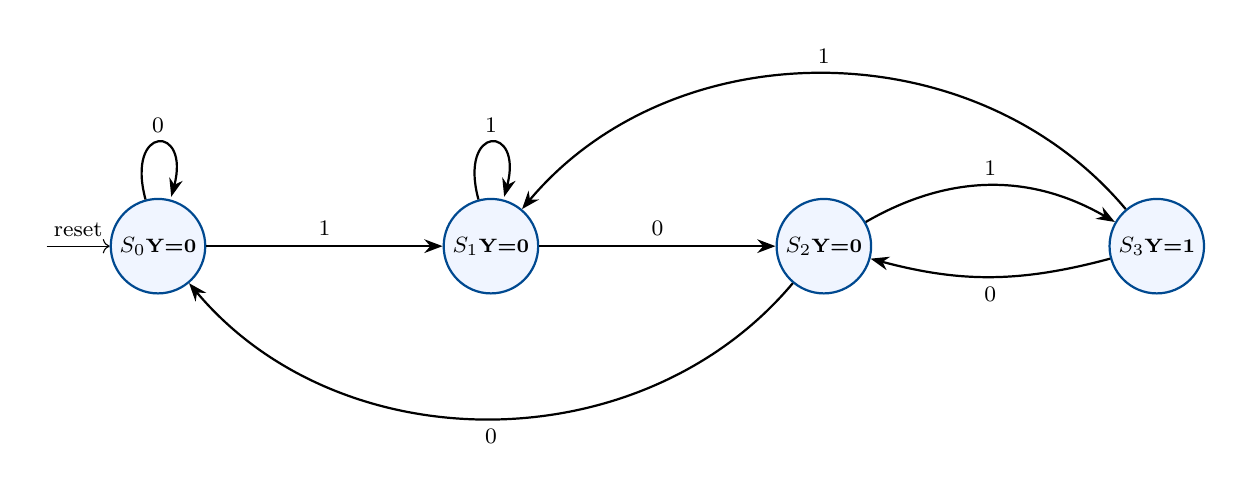
\begin{tikzpicture}[node distance=3cm]
  \node[reset] (start) {};
  \node[state, right=0.8cm of start] (S0) {$S_0$\\{\scriptsize Y=0}};
  \node[state, right=of S0] (S1) {$S_1$\\{\scriptsize Y=0}};
  \node[state, right=of S1] (S2) {$S_2$\\{\scriptsize Y=0}};
  \node[state, right=of S2] (S3) {$S_3$\\{\scriptsize Y=1}};

  \draw[->] (start) -- (S0) node[midway, above]{\footnotesize reset};
  \path (S0) edge[loop above] node{0} ()
        (S0) edge node[above]{1} (S1)
        (S1) edge node[above]{0} (S2)
        (S1) edge[loop above] node{1} ()
        (S2) edge[bend left=30] node[above]{1} (S3)
        (S2) edge[bend left=50] node[below]{0} (S0)
        (S3) edge[bend left=15] node[below]{0} (S2)
        (S3) edge[bend right=50] node[above]{1} (S1);
\end{tikzpicture}
\caption{State Diagram for ``101'' Sequence Detector (Moore)}
\end{figure}

\subsubsection{Step 2: State Assignment}

With 4 states we need $\lceil\log_2 4\rceil = 2$ flip-flops ($Q_1, Q_0$).

\begin{table}[H]
\centering
\begin{tabular}{c|cc}
\toprule
State & $Q_1$ & $Q_0$ \\
\midrule
$S_0$ & 0 & 0 \\
$S_1$ & 0 & 1 \\
$S_2$ & 1 & 0 \\
$S_3$ & 1 & 1 \\
\bottomrule
\end{tabular}
\caption{State Encoding}
\end{table}

\subsubsection{Step 3: State / Transition Table}

\begin{table}[H]
\centering
\caption{State Transition Table}
\begin{tabular}{cc|cc|c}
\toprule
\multicolumn{2}{c|}{Present State} & \multicolumn{2}{c|}{Next State} & Output \\
$Q_1 Q_0$ & $X$ & $Q_1^+ Q_0^+$ & State & $Y$ \\
\midrule
00 ($S_0$) & 0 & 00 & $S_0$ & 0 \\
00 ($S_0$) & 1 & 01 & $S_1$ & 0 \\
01 ($S_1$) & 0 & 10 & $S_2$ & 0 \\
01 ($S_1$) & 1 & 01 & $S_1$ & 0 \\
10 ($S_2$) & 0 & 00 & $S_0$ & 0 \\
10 ($S_2$) & 1 & 11 & $S_3$ & 0 \\
11 ($S_3$) & 0 & 10 & $S_2$ & 1 \\
11 ($S_3$) & 1 & 01 & $S_1$ & 1 \\
\bottomrule
\end{tabular}
\end{table}

\subsubsection{Step 4: Excitation Table (D Flip-Flops)}

Since $D = Q^+$, the excitation table is straightforward:

\begin{table}[H]
\centering
\caption{Excitation Table for D Flip-Flops}
\begin{tabular}{ccc|cc|cc}
\toprule
$Q_1$ & $Q_0$ & $X$ & $Q_1^+$ & $Q_0^+$ & $D_1$ & $D_0$ \\
\midrule
0 & 0 & 0 & 0 & 0 & 0 & 0 \\
0 & 0 & 1 & 0 & 1 & 0 & 1 \\
0 & 1 & 0 & 1 & 0 & 1 & 0 \\
0 & 1 & 1 & 0 & 1 & 0 & 1 \\
1 & 0 & 0 & 0 & 0 & 0 & 0 \\
1 & 0 & 1 & 1 & 1 & 1 & 1 \\
1 & 1 & 0 & 1 & 0 & 1 & 0 \\
1 & 1 & 1 & 0 & 1 & 0 & 1 \\
\bottomrule
\end{tabular}
\end{table}

\subsubsection{Step 5: K-Map Simplification}

\textbf{For $D_1$:}

\begin{figure}[H]
\centering
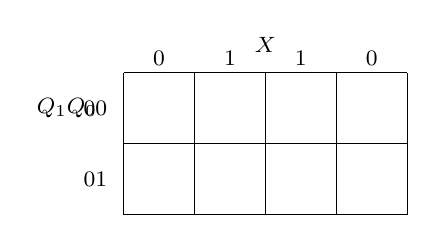
\begin{tikzpicture}[scale=0.9]
  % K-map for D1
  \draw (0,0) grid (4,2);
  \node at (-0.8,1.5) {\footnotesize $Q_1 Q_0$};
  \node at (2,2.4) {\footnotesize $X$};
  \node at (0.5,2.2) {\footnotesize 0};
  \node at (1.5,2.2) {\footnotesize 1};
  \node at (2.5,2.2) {\footnotesize 1};
  \node at (3.5,2.2) {\footnotesize 0};

  \node at (-0.4,1.5) {\footnotesize 00};
  \node at (-0.4,0.5) {\footnotesize 01};

  % Wait, K-map for 3 variables Q1, Q0, X
  % Let me redo this properly
\end{tikzpicture}
\end{figure}

K-map for $D_1$ with variables $Q_1, Q_0, X$:

\begin{table}[H]
\centering
\begin{tabular}{c|cc}
\toprule
$Q_1 Q_0 \backslash X$ & 0 & 1 \\
\midrule
00 & 0 & 0 \\
01 & 1 & 0 \\
11 & 1 & 0 \\
10 & 0 & 1 \\
\bottomrule
\end{tabular}
\quad\quad
\begin{tabular}{c|cc}
\toprule
$Q_1 Q_0 \backslash X$ & 0 & 1 \\
\midrule
00 & 0 & 1 \\
01 & 0 & 1 \\
11 & 0 & 1 \\
10 & 0 & 1 \\
\bottomrule
\end{tabular}

\vspace{0.3cm}
\hspace{1cm} K-map for $D_1$ \hspace{3cm} K-map for $D_0$
\end{table}

From the K-maps:
\begin{align}
D_1 &= Q_0 \cdot \overline{X} + Q_1 \cdot X \cdot \overline{Q_0} = Q_0\,\overline{X} + Q_1\,\overline{Q_0}\,X \\
D_0 &= X \\
Y &= Q_1 \cdot Q_0
\end{align}

\subsubsection{Step 6: Circuit Diagram}

\begin{figure}[H]
\centering
\begin{tikzpicture}[
  block/.style={draw, thick, minimum width=1.5cm, minimum height=1.8cm, fill=lightbg},
  gate/.style={draw, thick, minimum size=0.8cm},
  >=Stealth, scale=0.9, every node/.style={scale=0.9}
]
  % D Flip-Flops
  \node[block] (FF1) at (8,3) {$D_1$\\FF};
  \node[block] (FF0) at (8,0) {$D_0$\\FF};

  % Inputs
  \node at (-1,0) (Xin) {$X$};

  % D1 = Q0·X' + Q1·Q0'·X
  \node[draw, thick, minimum width=1cm, minimum height=0.6cm] (AND1) at (4,4) {AND};
  \node[draw, thick, minimum width=1cm, minimum height=0.6cm] (AND2) at (4,2.5) {AND};
  \node[draw, thick, minimum width=1cm, minimum height=0.6cm] (OR1) at (6,3) {OR};
  \node[draw, thick, minimum width=1cm, minimum height=0.6cm] (AND3) at (12,1.5) {AND};

  % Connections for D1
  \draw[->] (AND1.east) -- (OR1.west |- 4,3.2) -- (OR1.170);
  \draw[->] (AND2.east) -- (OR1.west |- 2.5,2.8) -- (OR1.190);
  \draw[->] (OR1.east) -- (FF1.west);

  % D0 = X
  \draw[->] (Xin) -- (FF0.west) node[midway, above]{\footnotesize $D_0 = X$};

  % Outputs from FFs
  \draw[->] (FF1.east) -- ++(1,0) node[right]{$Q_1$};
  \draw[->] (FF0.east) -- ++(1,0) node[right]{$Q_0$};

  % AND gate for output
  \draw[->] (AND3.east) -- ++(1,0) node[right]{$Y = Q_1 \cdot Q_0$};

  % Labels
  \node[above=0.1cm of FF1] {\footnotesize CLK $\uparrow$};
  \node[above=0.1cm of FF0] {\footnotesize CLK $\uparrow$};

  % Annotation
  \node[draw, dashed, rounded corners, fit=(AND1)(AND2)(OR1), inner sep=0.3cm, label=above:{\footnotesize $D_1 = Q_0\overline{X} + Q_1\overline{Q_0}X$}] {};
\end{tikzpicture}
\caption{Circuit Implementation for ``101'' Detector}
\end{figure}


% ══════════════════════════════════════════════════════════════════
\section{FSM Design Problems: Beginner to Advanced}
% ══════════════════════════════════════════════════════════════════

% ────────────────────────────────────────────────────
\subsection{Problem 1: Simple Toggle Switch (Beginner)}
% ────────────────────────────────────────────────────

\begin{infobox}[Problem Statement]
Design a Moore FSM with one input $T$ and one output $Y$. The output toggles (changes state) every time $T=1$ on a clock edge. When $T=0$, output remains unchanged. Initial output = 0.
\end{infobox}

\textbf{State Diagram:}

\begin{figure}[H]
\centering
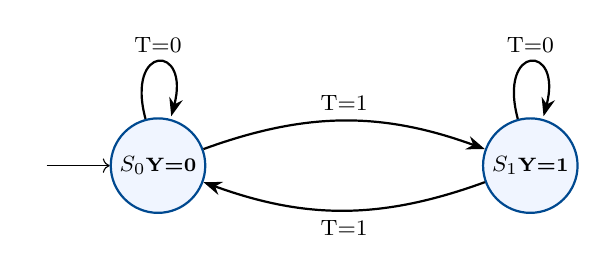
\begin{tikzpicture}[node distance=3.5cm]
  \node[reset] (start) {};
  \node[state, right=0.8cm of start] (S0) {$S_0$\\{\scriptsize Y=0}};
  \node[state, right=of S0] (S1) {$S_1$\\{\scriptsize Y=1}};

  \draw[->] (start) -- (S0);
  \path (S0) edge[bend left=20] node[above]{T=1} (S1)
        (S1) edge[bend left=20] node[below]{T=1} (S0)
        (S0) edge[loop above] node{T=0} ()
        (S1) edge[loop above] node{T=0} ();
\end{tikzpicture}
\caption{Toggle Switch FSM}
\end{figure}

\textbf{State Assignment:} $S_0 = 0$, $S_1 = 1$ (1 flip-flop $Q$)

\textbf{Transition \& Excitation Table:}

\begin{table}[H]
\centering
\begin{tabular}{cc|c|c|c}
\toprule
$Q$ & $T$ & $Q^+$ & $D$ & $Y$ \\
\midrule
0 & 0 & 0 & 0 & 0 \\
0 & 1 & 1 & 1 & 0 \\
1 & 0 & 1 & 1 & 1 \\
1 & 1 & 0 & 0 & 1 \\
\bottomrule
\end{tabular}
\end{table}

\textbf{Equations:}
\[
D = Q \oplus T = Q\,\overline{T} + \overline{Q}\,T, \quad Y = Q
\]


% ────────────────────────────────────────────────────
\subsection{Problem 2: 2-Bit Up Counter (Beginner)}
% ────────────────────────────────────────────────────

\begin{infobox}[Problem Statement]
Design a 2-bit binary up counter that counts 00 $\to$ 01 $\to$ 10 $\to$ 11 $\to$ 00 on each clock edge. Output is the count value.
\end{infobox}

\textbf{State Diagram:}

\begin{figure}[H]
\centering
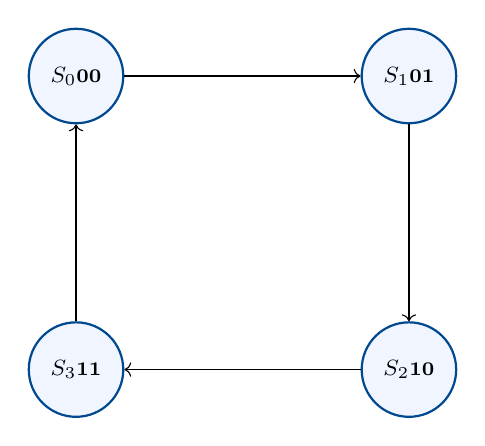
\begin{tikzpicture}[node distance=3cm]
  \node[state] (S0) {$S_0$\\{\scriptsize 00}};
  \node[state, right=of S0] (S1) {$S_1$\\{\scriptsize 01}};
  \node[state, below=2.5cm of S1] (S2) {$S_2$\\{\scriptsize 10}};
  \node[state, below=2.5cm of S0] (S3) {$S_3$\\{\scriptsize 11}};

  \draw[->] (S0) -- (S1);
  \draw[->] (S1) -- (S2);
  \draw[->] (S2) -- (S3);
  \draw[->] (S3) -- (S0);
\end{tikzpicture}
\caption{2-Bit Up Counter}
\end{figure}

\textbf{Excitation Table (no external input):}

\begin{table}[H]
\centering
\begin{tabular}{cc|cc|cc}
\toprule
$Q_1$ & $Q_0$ & $Q_1^+$ & $Q_0^+$ & $D_1$ & $D_0$ \\
\midrule
0 & 0 & 0 & 1 & 0 & 1 \\
0 & 1 & 1 & 0 & 1 & 0 \\
1 & 0 & 1 & 1 & 1 & 1 \\
1 & 1 & 0 & 0 & 0 & 0 \\
\bottomrule
\end{tabular}
\end{table}

\textbf{Equations:}
\[
D_1 = Q_1 \oplus Q_0, \quad D_0 = \overline{Q_0}
\]


% ────────────────────────────────────────────────────
\subsection{Problem 3: Sequence Detector ``11'' (Beginner)}
% ────────────────────────────────────────────────────

\begin{infobox}[Problem Statement]
Design a Mealy FSM that outputs 1 when two consecutive 1's are detected on input $X$. Overlapping allowed.
\end{infobox}

\textbf{State Diagram:}

\begin{figure}[H]
\centering
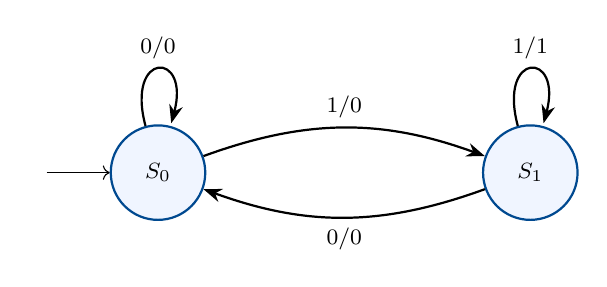
\begin{tikzpicture}[node distance=3.5cm]
  \node[reset] (start) {};
  \node[state, right=0.8cm of start] (S0) {$S_0$};
  \node[state, right=of S0] (S1) {$S_1$};

  \draw[->] (start) -- (S0);
  \path (S0) edge[bend left=20] node[above]{1/0} (S1)
        (S0) edge[loop above] node{0/0} ()
        (S1) edge[loop above] node{1/1} ()
        (S1) edge[bend left=20] node[below]{0/0} (S0);
\end{tikzpicture}
\caption{``11'' Sequence Detector (Mealy)}
\end{figure}

\textbf{State Assignment:} $S_0 = 0$, $S_1 = 1$

\textbf{Excitation Table:}

\begin{table}[H]
\centering
\begin{tabular}{cc|c|c|c}
\toprule
$Q$ & $X$ & $Q^+$ & $D$ & $Y$ \\
\midrule
0 & 0 & 0 & 0 & 0 \\
0 & 1 & 1 & 1 & 0 \\
1 & 0 & 0 & 0 & 0 \\
1 & 1 & 1 & 1 & 1 \\
\bottomrule
\end{tabular}
\end{table}

\textbf{Equations:}
\[
D = X, \quad Y = Q \cdot X
\]


% ────────────────────────────────────────────────────
\subsection{Problem 4: 3-Bit Up/Down Counter (Beginner--Intermediate)}
% ────────────────────────────────────────────────────

\begin{infobox}[Problem Statement]
Design a 3-bit counter with input $M$: counts up when $M=1$, counts down when $M=0$.
\end{infobox}

\textbf{State Diagram:}

\begin{figure}[H]
\centering
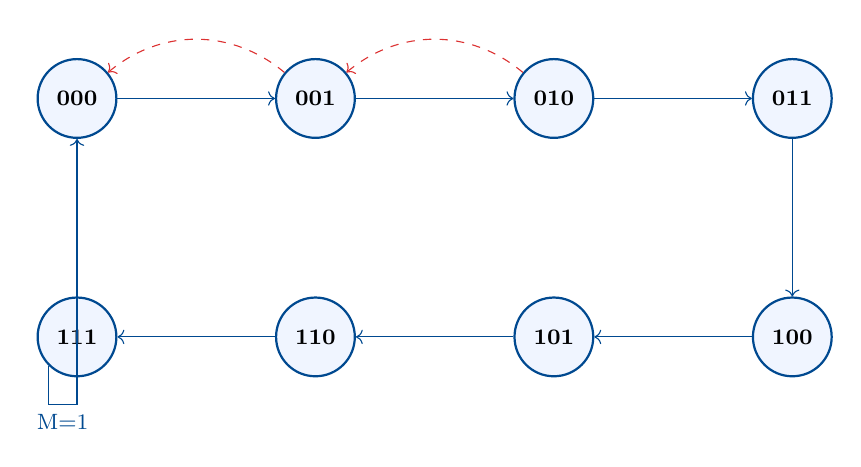
\begin{tikzpicture}[node distance=2cm, state/.append style={minimum size=1cm}]
  \node[state] (S0) {000};
  \node[state, right=of S0] (S1) {001};
  \node[state, right=of S1] (S2) {010};
  \node[state, right=of S2] (S3) {011};
  \node[state, below=of S3] (S4) {100};
  \node[state, left=of S4] (S5) {101};
  \node[state, left=of S5] (S6) {110};
  \node[state, left=of S6] (S7) {111};

  % Up direction (M=1)
  \draw[->, color=primary] (S0) -- (S1);
  \draw[->, color=primary] (S1) -- (S2);
  \draw[->, color=primary] (S2) -- (S3);
  \draw[->, color=primary] (S3) -- (S4);
  \draw[->, color=primary] (S4) -- (S5);
  \draw[->, color=primary] (S5) -- (S6);
  \draw[->, color=primary] (S6) -- (S7);
  \draw[->, color=primary] (S7.south west) -- ++(0,-0.5) -| (S0.south) node[near start, below]{\footnotesize\color{primary} M=1};

  % Down direction arrows (M=0)
  \draw[->, color=accent, dashed, bend right=40] (S1) to (S0);
  \draw[->, color=accent, dashed, bend right=40] (S2) to (S1);
\end{tikzpicture}
\caption{3-Bit Up/Down Counter (blue=up M=1, red dashed=down M=0)}
\end{figure}

\textbf{Equations (derived from standard counter logic):}
\begin{align}
D_2 &= Q_2 \oplus (M \cdot Q_1 \cdot Q_0 + \overline{M} \cdot \overline{Q_1} \cdot \overline{Q_0}) \\
D_1 &= Q_1 \oplus (M \cdot Q_0 + \overline{M} \cdot \overline{Q_0}) \\
D_0 &= \overline{Q_0}
\end{align}


% ────────────────────────────────────────────────────
\subsection{Problem 5: Vending Machine Controller (Intermediate)}
% ────────────────────────────────────────────────────

\begin{infobox}[Problem Statement]
Design a Moore FSM for a vending machine that accepts 5¢ and 10¢ coins. Item costs 15¢. Output \texttt{DISPENSE}=1 when 15¢ or more is collected, then reset. No change given.
\end{infobox}

\textbf{States:}
$S_0$: 0¢, \; $S_1$: 5¢, \; $S_2$: 10¢, \; $S_3$: 15¢+ (dispense)

\textbf{Inputs:} $N$ (nickel=5¢), $D$ (dime=10¢). Assume mutually exclusive.

\begin{figure}[H]
\centering
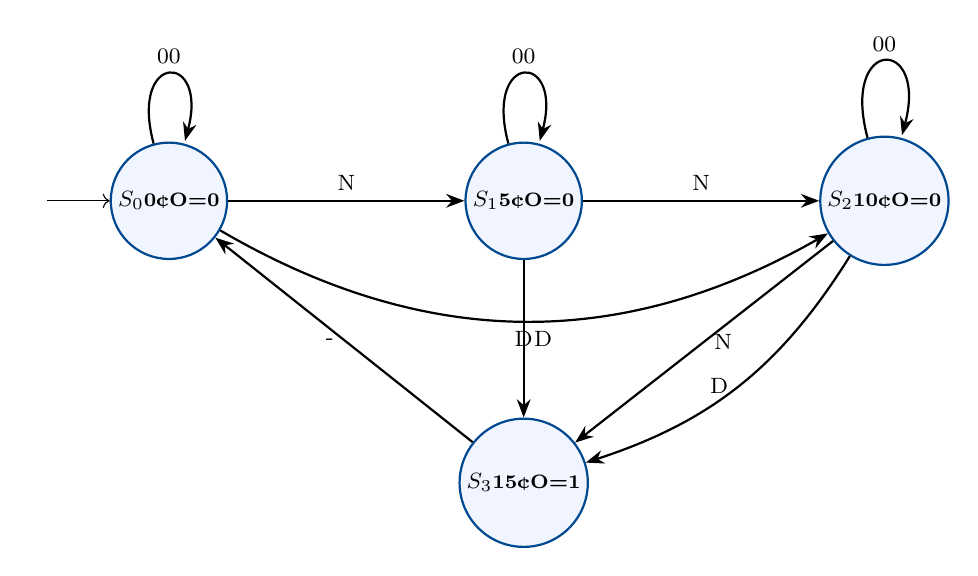
\begin{tikzpicture}[node distance=3cm]
  \node[reset] (start) {};
  \node[state, right=0.8cm of start] (S0) {$S_0$\\{\scriptsize 0¢}\\{\scriptsize O=0}};
  \node[state, right=of S0] (S1) {$S_1$\\{\scriptsize 5¢}\\{\scriptsize O=0}};
  \node[state, right=of S1] (S2) {$S_2$\\{\scriptsize 10¢}\\{\scriptsize O=0}};
  \node[state, below=2cm of S1] (S3) {$S_3$\\{\scriptsize 15¢}\\{\scriptsize O=1}};

  \draw[->] (start) -- (S0);
  \path (S0) edge node[above]{N} (S1)
        (S0) edge[bend right=30] node[below]{D} (S2)
        (S1) edge node[above]{N} (S2)
        (S1) edge node[right]{D} (S3)
        (S2) edge node[right]{N} (S3)
        (S2) edge[bend left=20] node[left]{D} (S3)
        (S3) edge node[left]{-} (S0)
        (S0) edge[loop above] node{00} ()
        (S1) edge[loop above] node{00} ()
        (S2) edge[loop above] node{00} ();
\end{tikzpicture}
\caption{Vending Machine FSM}
\end{figure}

\textbf{State Assignment:} $S_0=00$, $S_1=01$, $S_2=10$, $S_3=11$

\textbf{Transition Table:}

\begin{table}[H]
\centering
\begin{tabular}{cc|cc|cc|c}
\toprule
$Q_1$ & $Q_0$ & $N$ & $D$ & $Q_1^+$ & $Q_0^+$ & Dispense \\
\midrule
0 & 0 & 0 & 0 & 0 & 0 & 0 \\
0 & 0 & 1 & 0 & 0 & 1 & 0 \\
0 & 0 & 0 & 1 & 1 & 0 & 0 \\
0 & 1 & 0 & 0 & 0 & 1 & 0 \\
0 & 1 & 1 & 0 & 1 & 0 & 0 \\
0 & 1 & 0 & 1 & 1 & 1 & 0 \\
1 & 0 & 0 & 0 & 1 & 0 & 0 \\
1 & 0 & 1 & 0 & 1 & 1 & 0 \\
1 & 0 & 0 & 1 & 1 & 1 & 0 \\
1 & 1 & X & X & 0 & 0 & 1 \\
\bottomrule
\end{tabular}
\end{table}

\textbf{Equations (simplified):}
\begin{align}
D_1 &= Q_1\,\overline{Q_0} + \overline{Q_1}\,Q_0\,N + \overline{Q_1}\,D + Q_1\,Q_0' \cdot(N+D) \\
D_0 &= \overline{Q_1}\,\overline{Q_0}\,N + \overline{Q_1}\,Q_0\,\overline{N}\,\overline{D} + Q_1\,\overline{Q_0}\,(N+D) + \overline{Q_1}\,Q_0\,D \\
\text{Dispense} &= Q_1 \cdot Q_0
\end{align}


% ────────────────────────────────────────────────────
\subsection{Problem 6: Traffic Light Controller (Intermediate)}
% ────────────────────────────────────────────────────

\begin{infobox}[Problem Statement]
Design a Moore FSM for a simple traffic light: Green (G) $\to$ Yellow (Y) $\to$ Red (R) $\to$ Green. Each state lasts one clock period. A sensor input $S$ keeps green as long as $S=1$ (cars present).
\end{infobox}

\textbf{States:} $S_G$ (Green), $S_Y$ (Yellow), $S_R$ (Red)

\begin{figure}[H]
\centering
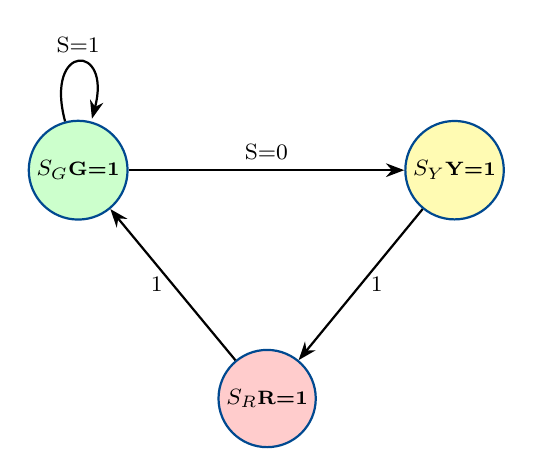
\begin{tikzpicture}[node distance=3.5cm]
  \node[state, fill=green!20] (SG) {$S_G$\\{\scriptsize G=1}};
  \node[state, fill=yellow!30, right=of SG] (SY) {$S_Y$\\{\scriptsize Y=1}};
  \node[state, fill=red!20, below right=2cm and 1.5cm of SG] (SR) {$S_R$\\{\scriptsize R=1}};

  \path (SG) edge[loop above] node{S=1} ()
        (SG) edge node[above]{S=0} (SY)
        (SY) edge node[right]{1} (SR)
        (SR) edge node[left]{1} (SG);
\end{tikzpicture}
\caption{Traffic Light Controller}
\end{figure}

\textbf{State Assignment:} $S_G=00$, $S_Y=01$, $S_R=10$

\textbf{Excitation Table:}

\begin{table}[H]
\centering
\begin{tabular}{ccc|cc|cc|ccc}
\toprule
$Q_1$ & $Q_0$ & $S$ & $Q_1^+$ & $Q_0^+$ & $D_1$ & $D_0$ & G & Y & R \\
\midrule
0 & 0 & 0 & 0 & 1 & 0 & 1 & 1 & 0 & 0 \\
0 & 0 & 1 & 0 & 0 & 0 & 0 & 1 & 0 & 0 \\
0 & 1 & X & 1 & 0 & 1 & 0 & 0 & 1 & 0 \\
1 & 0 & X & 0 & 0 & 0 & 0 & 0 & 0 & 1 \\
1 & 1 & X & 0 & 0 & 0 & 0 & -- & -- & -- \\
\bottomrule
\end{tabular}
\end{table}

\textbf{Equations:}
\begin{align}
D_1 &= Q_0 \\
D_0 &= \overline{Q_1} \cdot \overline{Q_0} \cdot \overline{S} \\
G &= \overline{Q_1} \cdot \overline{Q_0}, \quad Y = \overline{Q_1} \cdot Q_0, \quad R = Q_1 \cdot \overline{Q_0}
\end{align}


% ────────────────────────────────────────────────────
\subsection{Problem 7: Serial Adder (Intermediate)}
% ────────────────────────────────────────────────────

\begin{infobox}[Problem Statement]
Design a Mealy FSM serial adder. Two serial inputs $A$ and $B$ (LSB first) are added bit by bit. The FSM stores carry as state. Output $S$ = sum bit.
\end{infobox}

\textbf{States:} $S_0$ (carry = 0), $S_1$ (carry = 1)

\begin{figure}[H]
\centering
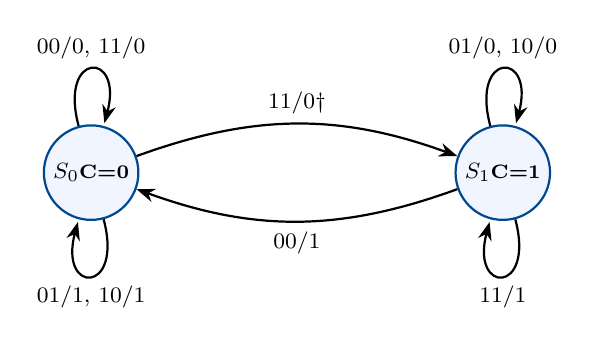
\begin{tikzpicture}[node distance=4cm]
  \node[state] (C0) {$S_0$\\{\scriptsize C=0}};
  \node[state, right=of C0] (C1) {$S_1$\\{\scriptsize C=1}};

  \path (C0) edge[loop above] node{00/0, 11/0} ()
        (C0) edge[loop below] node{01/1, 10/1} ()
        (C0) edge[bend left=20] node[above]{11/0$\dagger$} (C1)
        (C1) edge[bend left=20] node[below]{00/1} (C0)
        (C1) edge[loop above] node{01/0, 10/0} ()
        (C1) edge[loop below] node{11/1} ();
\end{tikzpicture}
\caption{Serial Adder FSM --- $\dagger$ transitions corrected below}
\end{figure}

Full truth table for serial addition: $A + B + C_{in} = \{C_{out}, S\}$

\begin{table}[H]
\centering
\begin{tabular}{ccc|cc|c|c}
\toprule
$Q$ (C$_{in}$) & $A$ & $B$ & Sum & C$_{out}$ & $D$ & $S$ \\
\midrule
0 & 0 & 0 & 0 & 0 & 0 & 0 \\
0 & 0 & 1 & 1 & 0 & 0 & 1 \\
0 & 1 & 0 & 1 & 0 & 0 & 1 \\
0 & 1 & 1 & 0 & 1 & 1 & 0 \\
1 & 0 & 0 & 1 & 0 & 0 & 1 \\
1 & 0 & 1 & 0 & 1 & 1 & 0 \\
1 & 1 & 0 & 0 & 1 & 1 & 0 \\
1 & 1 & 1 & 1 & 1 & 1 & 1 \\
\bottomrule
\end{tabular}
\end{table}

\textbf{Equations:}
\begin{align}
D &= A \cdot B + A \cdot Q + B \cdot Q = \text{Majority}(A, B, Q) \\
S &= A \oplus B \oplus Q
\end{align}


% ────────────────────────────────────────────────────
\subsection{Problem 8: Pattern Detector ``1010'' Non-Overlapping (Intermediate)}
% ────────────────────────────────────────────────────

\begin{infobox}[Problem Statement]
Design a Moore FSM that detects the non-overlapping sequence ``1010'' on input $X$. Output $Y=1$ for one clock cycle upon detection.
\end{infobox}

\textbf{States:} $S_0$ (idle), $S_1$ (got 1), $S_2$ (got 10), $S_3$ (got 101), $S_4$ (got 1010, output)

\begin{figure}[H]
\centering
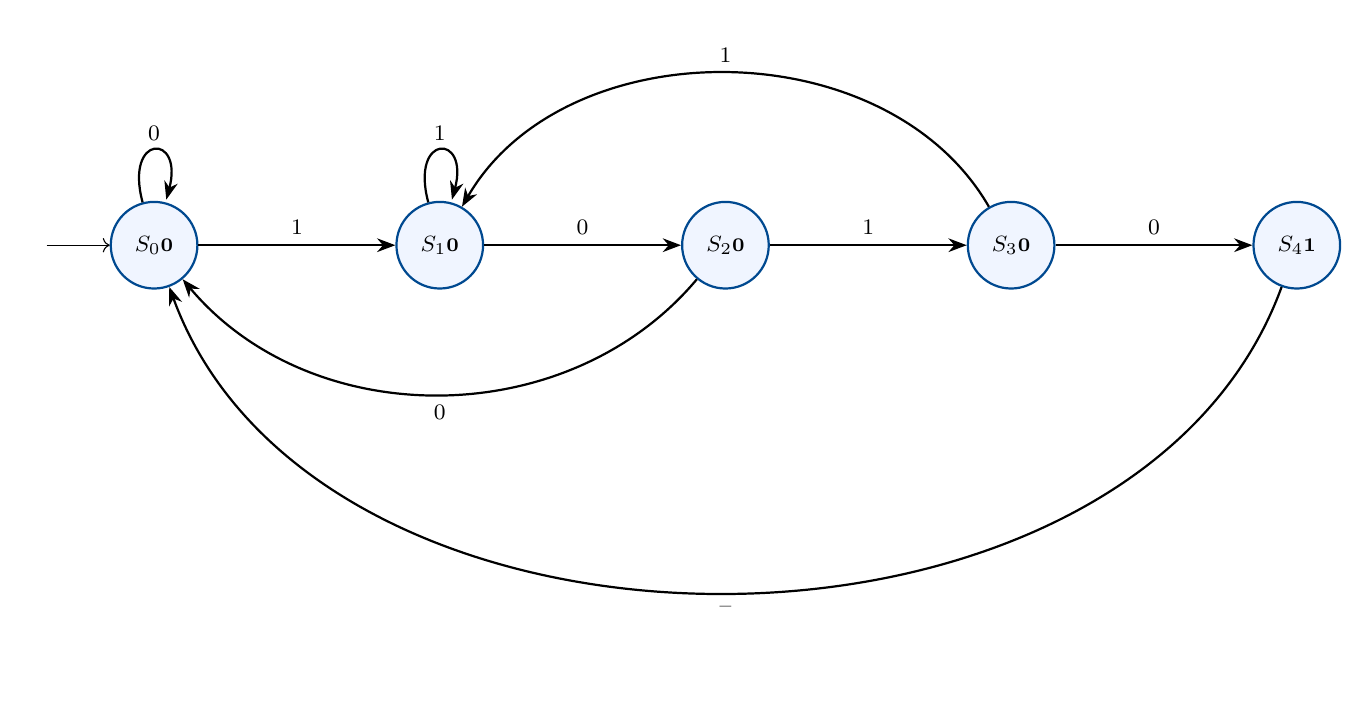
\begin{tikzpicture}[node distance=2.5cm, state/.append style={minimum size=1.1cm}]
  \node[reset] (start) {};
  \node[state, right=0.8cm of start] (S0) {$S_0$\\{\scriptsize 0}};
  \node[state, right=of S0] (S1) {$S_1$\\{\scriptsize 0}};
  \node[state, right=of S1] (S2) {$S_2$\\{\scriptsize 0}};
  \node[state, right=of S2] (S3) {$S_3$\\{\scriptsize 0}};
  \node[state, right=of S3] (S4) {$S_4$\\{\scriptsize 1}};

  \draw[->] (start) -- (S0);
  \path (S0) edge node[above]{1} (S1)
        (S0) edge[loop above] node{0} ()
        (S1) edge node[above]{0} (S2)
        (S1) edge[loop above] node{1} ()
        (S2) edge node[above]{1} (S3)
        (S2) edge[bend left=50] node[below]{0} (S0)
        (S3) edge node[above]{0} (S4)
        (S3) edge[bend right=60] node[above]{1} (S1)
        (S4) edge[bend left=70] node[below]{--} (S0);
\end{tikzpicture}
\caption{``1010'' Non-Overlapping Detector (Moore)}
\end{figure}

\textbf{State Assignment} (5 states $\Rightarrow$ 3 flip-flops):

\begin{table}[H]
\centering
\begin{tabular}{c|ccc}
\toprule
State & $Q_2$ & $Q_1$ & $Q_0$ \\
\midrule
$S_0$ & 0 & 0 & 0 \\
$S_1$ & 0 & 0 & 1 \\
$S_2$ & 0 & 1 & 0 \\
$S_3$ & 0 & 1 & 1 \\
$S_4$ & 1 & 0 & 0 \\
\bottomrule
\end{tabular}
\end{table}

\textbf{Excitation Table:}

\begin{table}[H]
\centering
\footnotesize
\begin{tabular}{cccc|ccc|ccc|c}
\toprule
$Q_2$ & $Q_1$ & $Q_0$ & $X$ & $Q_2^+$ & $Q_1^+$ & $Q_0^+$ & $D_2$ & $D_1$ & $D_0$ & $Y$ \\
\midrule
0 & 0 & 0 & 0 & 0 & 0 & 0 & 0 & 0 & 0 & 0 \\
0 & 0 & 0 & 1 & 0 & 0 & 1 & 0 & 0 & 1 & 0 \\
0 & 0 & 1 & 0 & 0 & 1 & 0 & 0 & 1 & 0 & 0 \\
0 & 0 & 1 & 1 & 0 & 0 & 1 & 0 & 0 & 1 & 0 \\
0 & 1 & 0 & 0 & 0 & 0 & 0 & 0 & 0 & 0 & 0 \\
0 & 1 & 0 & 1 & 0 & 1 & 1 & 0 & 1 & 1 & 0 \\
0 & 1 & 1 & 0 & 1 & 0 & 0 & 1 & 0 & 0 & 0 \\
0 & 1 & 1 & 1 & 0 & 0 & 1 & 0 & 0 & 1 & 0 \\
1 & 0 & 0 & X & 0 & 0 & 0 & 0 & 0 & 0 & 1 \\
\bottomrule
\end{tabular}
\end{table}

Unused states (101, 110, 111) $\to D_2 D_1 D_0 = 000$ (safe reset).

\textbf{Equations} (from K-maps):
\begin{align}
D_2 &= Q_1 \cdot Q_0 \cdot \overline{X} \\
D_1 &= Q_0 \cdot \overline{X} \cdot \overline{Q_1} + Q_1 \cdot \overline{Q_0} \cdot X \\
D_0 &= X \cdot \overline{Q_2} \cdot (\overline{Q_1} + \overline{Q_0} \cdot Q_1) = X \cdot \overline{Q_2} \cdot \overline{Q_1 \cdot Q_0}\\
Y &= Q_2
\end{align}


% ────────────────────────────────────────────────────
\subsection{Problem 9: Elevator Door Controller (Intermediate--Advanced)}
% ────────────────────────────────────────────────────

\begin{infobox}[Problem Statement]
Design a Moore FSM for an elevator door with inputs: $OPEN\_BTN$, $CLOSE\_BTN$, $SENSOR$ (obstacle detected). States: CLOSED, OPENING, OPEN, CLOSING.

Rules: (1) If obstacle detected while closing, go to OPENING. (2) Door stays open while OPEN\_BTN pressed. (3) After open completes, wait then close.
\end{infobox}

\begin{figure}[H]
\centering
\begin{tikzpicture}[node distance=3.5cm, state/.append style={minimum size=1.3cm}]
  \node[state, fill=red!10] (CL) {CLOSED\\{\scriptsize O=00}};
  \node[state, fill=green!10, right=of CL] (OP) {OPENING\\{\scriptsize O=01}};
  \node[state, fill=green!20, below=3cm of OP] (OPEN) {OPEN\\{\scriptsize O=10}};
  \node[state, fill=yellow!10, below=3cm of CL] (CLG) {CLOSING\\{\scriptsize O=11}};

  \path (CL) edge node[above]{OPEN\_BTN} (OP)
        (CL) edge[loop above] node{\overline{OPEN}} ()
        (OP) edge node[right]{done} (OPEN)
        (OP) edge[loop above] node{$\overline{done}$} ()
        (OPEN) edge node[below]{CLOSE\_BTN} (CLG)
        (OPEN) edge[loop below] node{OPEN\_BTN} ()
        (CLG) edge node[left]{done} (CL)
        (CLG) edge[bend left=15] node[right]{SENSOR} (OP)
        (CLG) edge[loop below] node{$\overline{done}\cdot\overline{SENSOR}$} ();
\end{tikzpicture}
\caption{Elevator Door Controller FSM}
\end{figure}

\textbf{State Assignment:} CLOSED=00, OPENING=01, OPEN=10, CLOSING=11.

The excitation and output equations follow from the standard derivation approach. The key insight here is the safety-critical transition: \textbf{CLOSING $\to$ OPENING} when sensor detects an obstacle takes priority over all other transitions.


% ────────────────────────────────────────────────────
\subsection{Problem 10: SPI Master Controller (Advanced)}
% ────────────────────────────────────────────────────

\begin{infobox}[Problem Statement]
Design a Moore FSM for a simplified SPI master that: (1) waits for a START signal, (2) asserts CS low, (3) shifts out 8 bits (MSB first) on MOSI with SCLK toggling, (4) de-asserts CS and returns to idle.
\end{infobox}

\textbf{States:}

\begin{figure}[H]
\centering
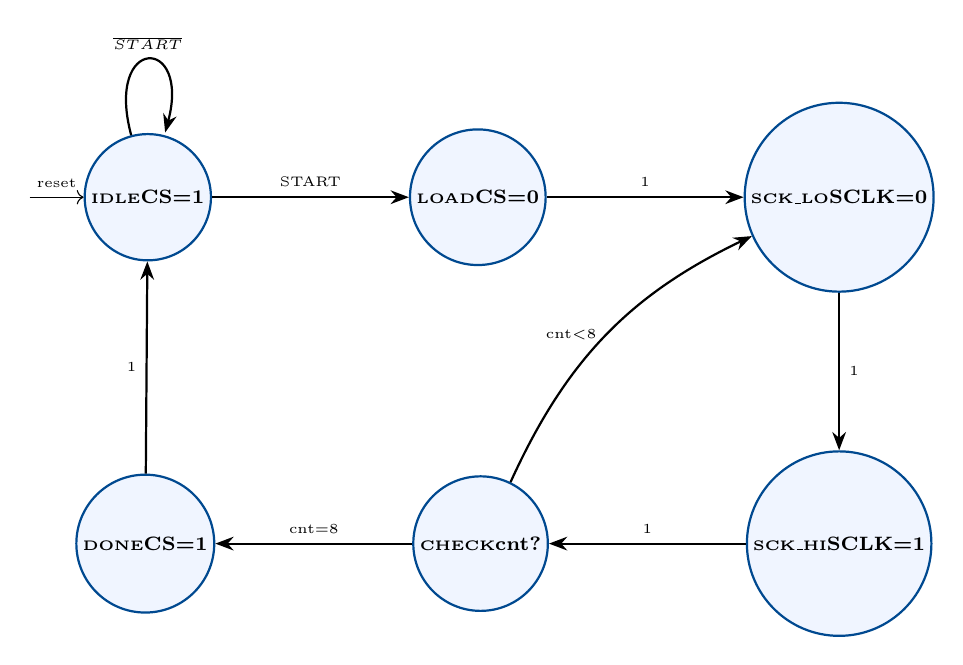
\begin{tikzpicture}[node distance=2.5cm, state/.append style={minimum size=1.2cm, font=\tiny\bfseries}]
  \node[state] (IDLE) {IDLE\\{\scriptsize CS=1}};
  \node[state, right=of IDLE] (LOAD) {LOAD\\{\scriptsize CS=0}};
  \node[state, right=of LOAD] (SCK_L) {SCK\_LO\\{\scriptsize SCLK=0}};
  \node[state, below=2cm of SCK_L] (SCK_H) {SCK\_HI\\{\scriptsize SCLK=1}};
  \node[state, left=of SCK_H] (CHECK) {CHECK\\{\scriptsize cnt?}};
  \node[state, left=of CHECK] (DONE) {DONE\\{\scriptsize CS=1}};

  \draw[->] (-1.5,0) -- (IDLE) node[midway, above]{\tiny reset};
  \path (IDLE) edge node[above]{\tiny START} (LOAD)
        (IDLE) edge[loop above] node{\tiny $\overline{START}$} ()
        (LOAD) edge node[above]{\tiny 1} (SCK_L)
        (SCK_L) edge node[right]{\tiny 1} (SCK_H)
        (SCK_H) edge node[above]{\tiny 1} (CHECK)
        (CHECK) edge[bend left=20] node[left]{\tiny cnt$<$8} (SCK_L)
        (CHECK) edge node[above]{\tiny cnt=8} (DONE)
        (DONE) edge node[left]{\tiny 1} (IDLE);
\end{tikzpicture}
\caption{SPI Master Controller FSM}
\end{figure}

This requires 6 states = 3 flip-flops + a 3-bit counter for bit count. The FSM controls the protocol while the counter tracks progress.


% ────────────────────────────────────────────────────
\subsection{Problem 11: UART Receiver (Advanced)}
% ────────────────────────────────────────────────────

\begin{infobox}[Problem Statement]
Design a Moore FSM for a UART receiver (8N1 format): detect start bit, sample 8 data bits at mid-bit, check stop bit, assert data-ready.
\end{infobox}

\begin{figure}[H]
\centering
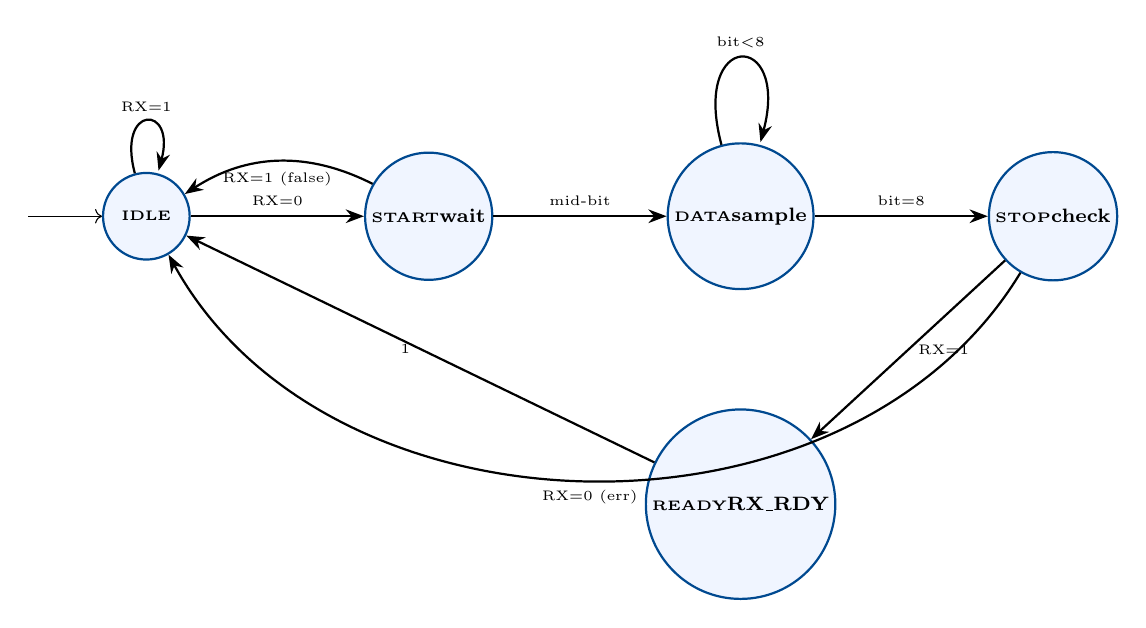
\begin{tikzpicture}[node distance=2.2cm, state/.append style={minimum size=1.1cm, font=\tiny\bfseries}]
  \node[state] (IDLE) {IDLE};
  \node[state, right=of IDLE] (START) {START\\{\scriptsize wait}};
  \node[state, right=of START] (DATA) {DATA\\{\scriptsize sample}};
  \node[state, right=of DATA] (STOP) {STOP\\{\scriptsize check}};
  \node[state, below=1.5cm of DATA] (READY) {READY\\{\scriptsize RX\_RDY}};

  \draw[->] (-1.5,0) -- (IDLE);
  \path (IDLE) edge node[above]{\tiny RX=0} (START)
        (IDLE) edge[loop above] node{\tiny RX=1} ()
        (START) edge node[above]{\tiny mid-bit} (DATA)
        (START) edge[bend right=30] node[below]{\tiny RX=1 (false)} (IDLE)
        (DATA) edge[loop above] node[above]{\tiny bit$<$8} ()
        (DATA) edge node[above]{\tiny bit=8} (STOP)
        (STOP) edge node[right]{\tiny RX=1} (READY)
        (STOP) edge[bend left=60] node[below]{\tiny RX=0 (err)} (IDLE)
        (READY) edge node[left]{\tiny 1} (IDLE);
\end{tikzpicture}
\caption{UART Receiver FSM}
\end{figure}

\textbf{Implementation notes:}
\begin{itemize}
  \item Requires a baud-rate counter (e.g., 16x oversampling) to find mid-bit timing
  \item 3-bit counter for tracking bit index (0--7)
  \item 8-bit shift register for received data
  \item 5 states $\to$ 3 flip-flops for state encoding
\end{itemize}


% ────────────────────────────────────────────────────
\subsection{Problem 12: Washing Machine Controller (Advanced)}
% ────────────────────────────────────────────────────

\begin{infobox}[Problem Statement]
Design a Moore FSM for a washing machine with states: IDLE, FILL, WASH, RINSE, SPIN, DONE. Inputs: START, WATER\_LEVEL, TIMER\_DONE. Outputs: VALVE, MOTOR, PUMP, BUZZER.
\end{infobox}

\begin{figure}[H]
\centering
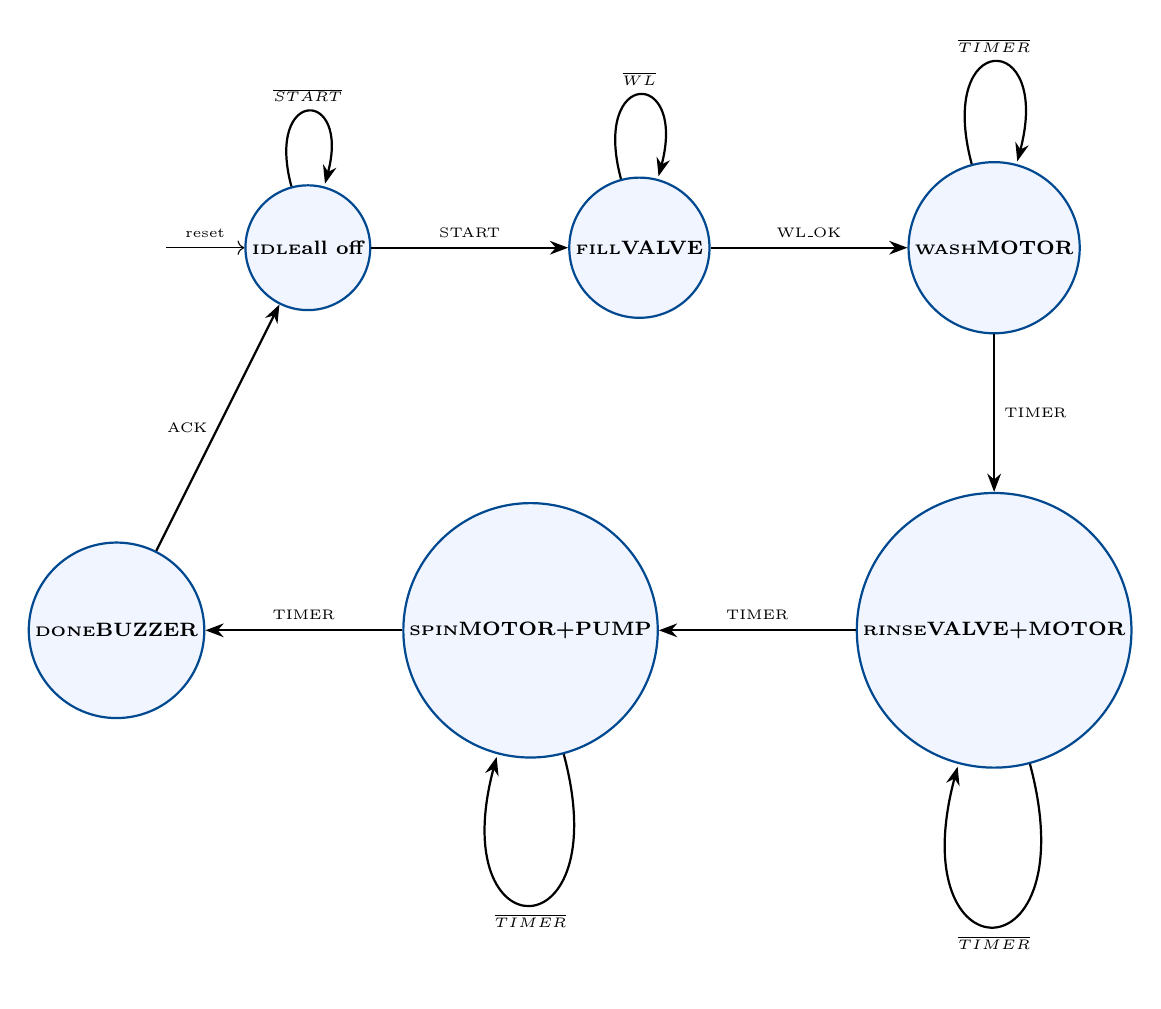
\begin{tikzpicture}[node distance=2cm, state/.append style={minimum size=1.1cm, font=\tiny\bfseries}]
  \node[state] (IDLE) {IDLE\\{\scriptsize all off}};
  \node[state, right=2.5cm of IDLE] (FILL) {FILL\\{\scriptsize VALVE}};
  \node[state, right=2.5cm of FILL] (WASH) {WASH\\{\scriptsize MOTOR}};
  \node[state, below=2cm of WASH] (RINSE) {RINSE\\{\scriptsize VALVE+\\MOTOR}};
  \node[state, left=2.5cm of RINSE] (SPIN) {SPIN\\{\scriptsize MOTOR+\\PUMP}};
  \node[state, left=2.5cm of SPIN] (DONE) {DONE\\{\scriptsize BUZZER}};

  \draw[->] (-1.8,0) -- (IDLE) node[midway, above]{\tiny reset};
  \path (IDLE) edge node[above]{\tiny START} (FILL)
        (IDLE) edge[loop above] node{\tiny $\overline{START}$} ()
        (FILL) edge node[above]{\tiny WL\_OK} (WASH)
        (FILL) edge[loop above] node{\tiny $\overline{WL}$} ()
        (WASH) edge node[right]{\tiny TIMER} (RINSE)
        (WASH) edge[loop above] node{\tiny $\overline{TIMER}$} ()
        (RINSE) edge node[above]{\tiny TIMER} (SPIN)
        (RINSE) edge[loop below] node{\tiny $\overline{TIMER}$} ()
        (SPIN) edge node[above]{\tiny TIMER} (DONE)
        (SPIN) edge[loop below] node{\tiny $\overline{TIMER}$} ()
        (DONE) edge node[left]{\tiny ACK} (IDLE);
\end{tikzpicture}
\caption{Washing Machine Controller FSM}
\end{figure}

\textbf{State Assignment} (6 states $\Rightarrow$ 3 flip-flops):

\begin{table}[H]
\centering
\begin{tabular}{c|ccc|cccc}
\toprule
State & $Q_2$ & $Q_1$ & $Q_0$ & VALVE & MOTOR & PUMP & BUZZER \\
\midrule
IDLE  & 0 & 0 & 0 & 0 & 0 & 0 & 0 \\
FILL  & 0 & 0 & 1 & 1 & 0 & 0 & 0 \\
WASH  & 0 & 1 & 0 & 0 & 1 & 0 & 0 \\
RINSE & 0 & 1 & 1 & 1 & 1 & 0 & 0 \\
SPIN  & 1 & 0 & 0 & 0 & 1 & 1 & 0 \\
DONE  & 1 & 0 & 1 & 0 & 0 & 0 & 1 \\
\bottomrule
\end{tabular}
\end{table}

\textbf{Output Equations:}
\begin{align}
\text{VALVE} &= Q_0 \cdot \overline{Q_2} \\
\text{MOTOR} &= Q_1 + Q_2\cdot\overline{Q_0} \\
\text{PUMP} &= Q_2 \cdot \overline{Q_1} \cdot \overline{Q_0} \\
\text{BUZZER} &= Q_2 \cdot Q_0
\end{align}


% ────────────────────────────────────────────────────
\subsection{Problem 13: Keypad Debouncer / Lock (Advanced)}
% ────────────────────────────────────────────────────

\begin{infobox}[Problem Statement]
Design a Mealy FSM for a 2-digit combination lock. The correct code is ``AB'' (two sequential inputs). If wrong digit entered at any stage, return to start. Output UNLOCK=1 only after correct sequence.
\end{infobox}

\begin{figure}[H]
\centering
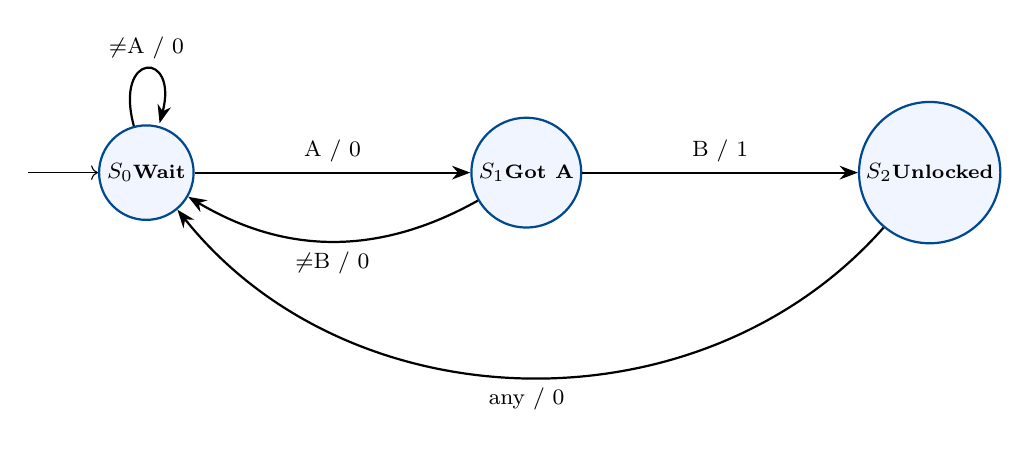
\begin{tikzpicture}[node distance=3.5cm]
  \node[state] (S0) {$S_0$\\{\scriptsize Wait}};
  \node[state, right=of S0] (S1) {$S_1$\\{\scriptsize Got A}};
  \node[state, right=of S1] (S2) {$S_2$\\{\scriptsize Unlocked}};

  \draw[->] (-1.5,0) -- (S0);
  \path (S0) edge node[above]{A / 0} (S1)
        (S0) edge[loop above] node{$\neq$A / 0} ()
        (S1) edge node[above]{B / 1} (S2)
        (S1) edge[bend left=30] node[below]{$\neq$B / 0} (S0)
        (S2) edge[bend left=50] node[below]{any / 0} (S0);
\end{tikzpicture}
\caption{Combination Lock FSM}
\end{figure}

With 3 states, we need 2 flip-flops. The input needs an encoder to convert keypad data to comparison signals.


% ────────────────────────────────────────────────────
\subsection{Problem 14: Memory Read Controller (Advanced)}
% ────────────────────────────────────────────────────

\begin{infobox}[Problem Statement]
Design a Moore FSM for a memory read controller that interfaces with SRAM. Sequence: IDLE $\to$ assert address and RD $\to$ wait for ACK $\to$ latch data $\to$ IDLE.
\end{infobox}

\begin{figure}[H]
\centering
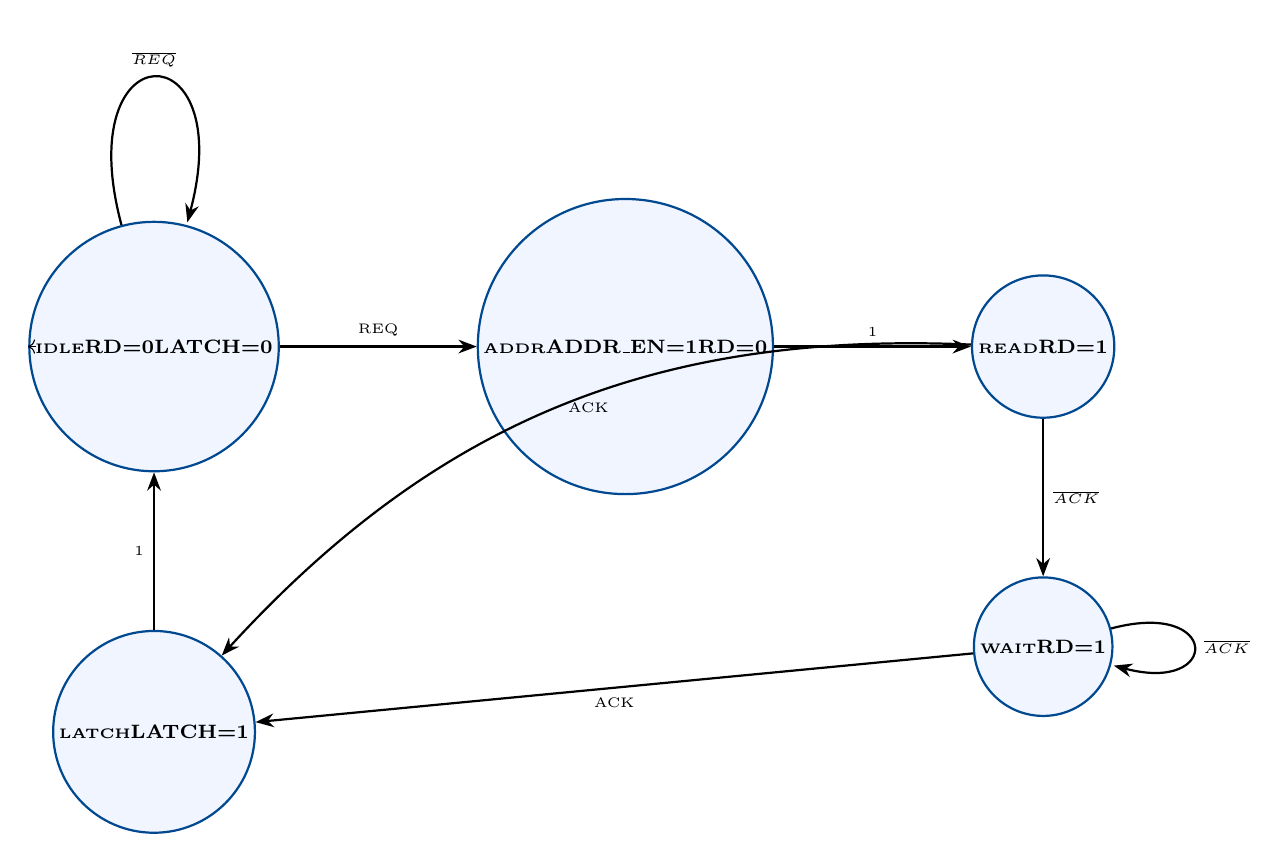
\begin{tikzpicture}[node distance=2.5cm, state/.append style={minimum size=1.2cm, font=\tiny\bfseries}]
  \node[state] (IDLE) {IDLE\\{\scriptsize RD=0\\LATCH=0}};
  \node[state, right=of IDLE] (ADDR) {ADDR\\{\scriptsize ADDR\_EN=1\\RD=0}};
  \node[state, right=of ADDR] (READ) {READ\\{\scriptsize RD=1}};
  \node[state, below=2cm of READ] (WAIT) {WAIT\\{\scriptsize RD=1}};
  \node[state, below=2cm of IDLE] (LATCH) {LATCH\\{\scriptsize LATCH=1}};

  \draw[->] (-1.5,0) -- (IDLE);
  \path (IDLE) edge node[above]{\tiny REQ} (ADDR)
        (IDLE) edge[loop above] node{\tiny $\overline{REQ}$} ()
        (ADDR) edge node[above]{\tiny 1} (READ)
        (READ) edge node[right]{\tiny $\overline{ACK}$} (WAIT)
        (READ) edge[bend right=25] node[right]{\tiny ACK} (LATCH)
        (WAIT) edge[loop right] node{\tiny $\overline{ACK}$} ()
        (WAIT) edge node[below]{\tiny ACK} (LATCH)
        (LATCH) edge node[left]{\tiny 1} (IDLE);
\end{tikzpicture}
\caption{Memory Read Controller FSM}
\end{figure}

\textbf{State Assignment} (5 states $\Rightarrow$ 3 flip-flops): IDLE=000, ADDR=001, READ=010, WAIT=011, LATCH=100.


% ────────────────────────────────────────────────────
\subsection{Problem 15: AHB-Lite Bus Master (Expert)}
% ────────────────────────────────────────────────────

\begin{infobox}[Problem Statement]
Design a Moore FSM for a simplified AHB-Lite bus master with pipelined transfers. States: IDLE, ADDR\_PHASE, DATA\_PHASE, WAIT\_HREADY, ERROR.

Inputs: HTRANS\_REQ, HREADY, HRESP.\\
Outputs: HTRANS[1:0], control signals.
\end{infobox}

\begin{figure}[H]
\centering
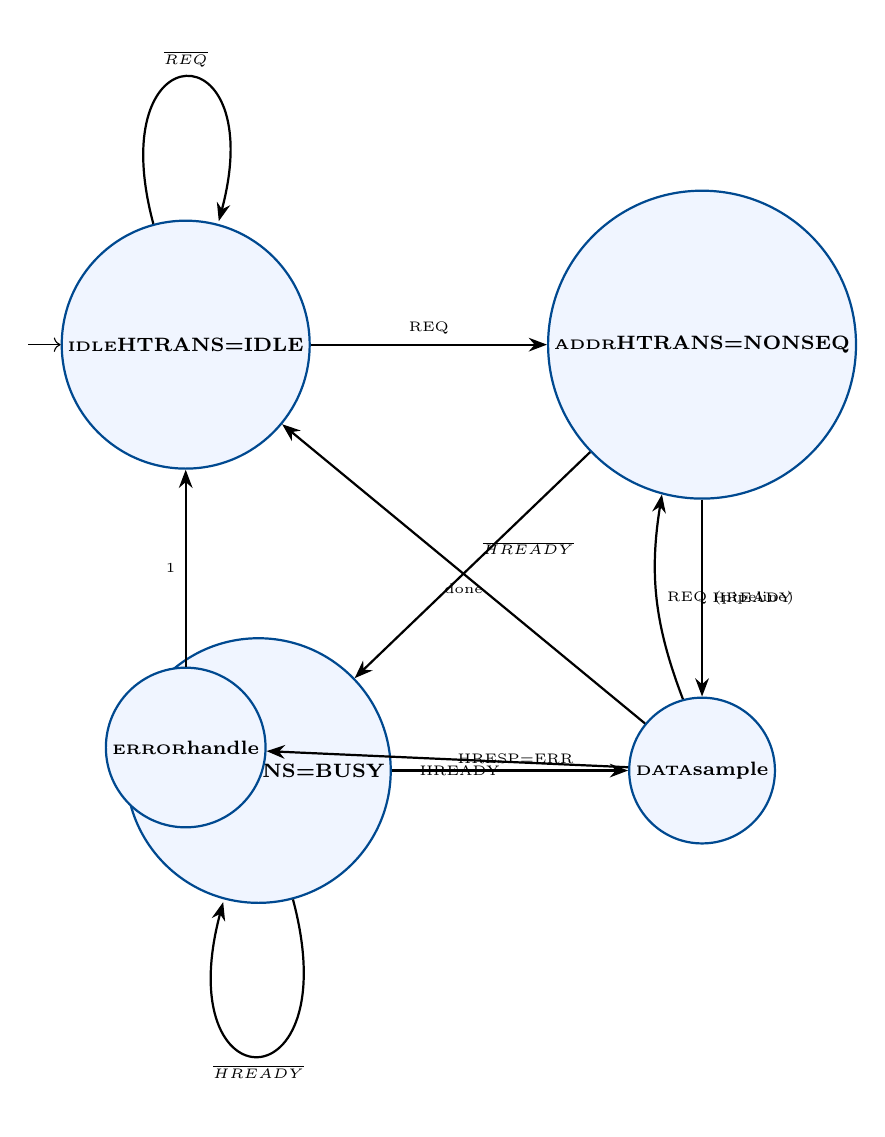
\begin{tikzpicture}[node distance=2.5cm, state/.append style={minimum size=1.3cm, font=\tiny\bfseries}]
  \node[state] (IDLE) {IDLE\\{\scriptsize HTRANS=\\IDLE}};
  \node[state, right=3cm of IDLE] (ADDR) {ADDR\\{\scriptsize HTRANS=\\NONSEQ}};
  \node[state, below=2.5cm of ADDR] (DATA) {DATA\\{\scriptsize sample}};
  \node[state, left=3cm of DATA] (WAIT) {WAIT\\{\scriptsize HTRANS=\\BUSY}};
  \node[state, below=2.5cm of IDLE] (ERR) {ERROR\\{\scriptsize handle}};

  \draw[->] (-2,0) -- (IDLE);
  \path (IDLE) edge node[above]{\tiny REQ} (ADDR)
        (IDLE) edge[loop above] node{\tiny $\overline{REQ}$} ()
        (ADDR) edge node[right]{\tiny HREADY} (DATA)
        (ADDR) edge node[above right]{\tiny $\overline{HREADY}$} (WAIT)
        (DATA) edge[bend left=15] node[right]{\tiny REQ (pipeline)} (ADDR)
        (DATA) edge node[below]{\tiny done} (IDLE)
        (DATA) edge node[right]{\tiny HRESP=ERR} (ERR)
        (WAIT) edge node[left]{\tiny HREADY} (DATA)
        (WAIT) edge[loop below] node{\tiny $\overline{HREADY}$} ()
        (ERR) edge node[left]{\tiny 1} (IDLE);
\end{tikzpicture}
\caption{AHB-Lite Bus Master FSM}
\end{figure}

\textbf{Key design considerations:}
\begin{itemize}
  \item Pipelined nature: address phase of next transfer overlaps data phase of current
  \item HREADY is critical --- FSM must stall when slave is not ready
  \item Error handling must comply with AMBA spec (two-cycle error response)
  \item 5 states $\to$ 3 flip-flops, but one-hot encoding preferred in FPGAs
\end{itemize}


% ══════════════════════════════════════════════════════════════════
\section{Complete Worked Example: Excitation Table to Circuit}
\label{sec:full_example}
% ══════════════════════════════════════════════════════════════════

Let us work through \textbf{Problem 6 (Traffic Light Controller)} completely.

\subsection{Given State Diagram}
Refer to Figure 8. States: $S_G=00$, $S_Y=01$, $S_R=10$. Input: $S$ (sensor). Unused: $11$.

\subsection{Complete Excitation Table}

\begin{table}[H]
\centering
\caption{Complete Traffic Light Excitation Table}
\begin{tabular}{ccc|cc|cc|ccc}
\toprule
$Q_1$ & $Q_0$ & $S$ & $Q_1^+$ & $Q_0^+$ & $D_1$ & $D_0$ & G & Y & R \\
\midrule
0 & 0 & 0 & 0 & 1 & 0 & 1 & 1 & 0 & 0 \\
0 & 0 & 1 & 0 & 0 & 0 & 0 & 1 & 0 & 0 \\
0 & 1 & 0 & 1 & 0 & 1 & 0 & 0 & 1 & 0 \\
0 & 1 & 1 & 1 & 0 & 1 & 0 & 0 & 1 & 0 \\
1 & 0 & 0 & 0 & 0 & 0 & 0 & 0 & 0 & 1 \\
1 & 0 & 1 & 0 & 0 & 0 & 0 & 0 & 0 & 1 \\
1 & 1 & 0 & 0 & 0 & 0 & 0 & d & d & d \\
1 & 1 & 1 & 0 & 0 & 0 & 0 & d & d & d \\
\bottomrule
\end{tabular}
\end{table}

\subsection{K-Map for $D_1$}

\begin{table}[H]
\centering
\begin{tabular}{c|cc}
& $S=0$ & $S=1$ \\
\midrule
$Q_1 Q_0 = 00$ & 0 & 0 \\
$Q_1 Q_0 = 01$ & \cellcolor{green!20}1 & \cellcolor{green!20}1 \\
$Q_1 Q_0 = 11$ & \cellcolor{gray!20}d & \cellcolor{gray!20}d \\
$Q_1 Q_0 = 10$ & 0 & 0 \\
\end{tabular}
\end{table}

Group: $Q_0 \cdot \overline{Q_1}$ (with don't-cares, can simplify to $Q_0$)

$$\boxed{D_1 = Q_0}$$

\subsection{K-Map for $D_0$}

\begin{table}[H]
\centering
\begin{tabular}{c|cc}
& $S=0$ & $S=1$ \\
\midrule
$Q_1 Q_0 = 00$ & \cellcolor{green!20}1 & 0 \\
$Q_1 Q_0 = 01$ & 0 & 0 \\
$Q_1 Q_0 = 11$ & \cellcolor{gray!20}d & \cellcolor{gray!20}d \\
$Q_1 Q_0 = 10$ & 0 & 0 \\
\end{tabular}
\end{table}

$$\boxed{D_0 = \overline{Q_1} \cdot \overline{Q_0} \cdot \overline{S}}$$

\subsection{Output K-Maps}

\textbf{Green} ($G = \overline{Q_1}\cdot\overline{Q_0}$), \textbf{Yellow} ($Y = \overline{Q_1}\cdot Q_0$), \textbf{Red} ($R = Q_1\cdot\overline{Q_0}$)

\subsection{Final Circuit}

\begin{figure}[H]
\centering
\begin{tikzpicture}[
  block/.style={draw, thick, minimum width=2cm, minimum height=1.4cm, fill=lightbg, font=\footnotesize},
  andg/.style={draw, thick, minimum width=1.2cm, minimum height=0.6cm, font=\scriptsize},
  inv/.style={draw, thick, circle, minimum size=0.4cm, font=\scriptsize, inner sep=1pt},
  >=Stealth, scale=0.85, every node/.style={scale=0.85}
]
  % Flip-flops
  \node[block] (FF1) at (6,4) {D FF\\$Q_1$};
  \node[block] (FF0) at (6,1) {D FF\\$Q_0$};

  % D1 = Q0
  \draw[->] (FF0.east) -- ++(1,0) |- ++(0,1.5) -- ++(-4.5,0) |- (FF1.west |- 4,4.3) node[near end, above]{\scriptsize $D_1 = Q_0$};

  % D0 = Q1' Q0' S'
  \node[andg] (A1) at (2,1) {AND3};
  \draw[->] (A1.east) -- (FF0.west) node[midway, above]{\scriptsize $D_0$};

  % Outputs
  \node[andg] (AG) at (11,5) {NOR};
  \node at (13,5) {G};
  \draw[->] (AG.east) -- (13,5);

  \node[andg] (AY) at (11,3.5) {AND};
  \node at (13,3.5) {Y};
  \draw[->] (AY.east) -- (13,3.5);

  \node[andg] (AR) at (11,2) {AND};
  \node at (13,2) {R};
  \draw[->] (AR.east) -- (13,2);

  % Q1 and Q0 outputs
  \draw[->] (FF1.east) -- ++(0.5,0) coordinate (q1out);
  \draw[->] (FF0.east) -- ++(0.5,0) coordinate (q0out);

  % Input
  \node at (-0.5,1) {$S$};

  % CLK
  \node at (6,6) {CLK};
  \draw[->] (6,5.8) -- (FF1.north);
  \draw[->] (6,5.8) -- ++(0,-2.8) -- (FF0.north);

  % Annotations
  \node[draw, dashed, rounded corners, inner sep=0.5cm, fit=(FF1)(FF0), label=above:State Register] {};
\end{tikzpicture}
\caption{Complete Traffic Light Controller Circuit}
\end{figure}


% ══════════════════════════════════════════════════════════════════
\section{Comparison: Moore vs.\ Mealy Implementation}
% ══════════════════════════════════════════════════════════════════

\begin{table}[H]
\centering
\caption{Moore vs.\ Mealy --- Design Trade-offs}
\begin{tabular}{p{3.5cm}p{5cm}p{5cm}}
\toprule
\textbf{Aspect} & \textbf{Moore} & \textbf{Mealy} \\
\midrule
Output depends on & State only & State + Input \\
\# States & Generally more & Generally fewer \\
Output timing & Changes with clock & Can change with input (async) \\
Glitch risk & Lower (synchronous) & Higher (input-dependent) \\
Output latency & One clock cycle more & Immediate \\
Design complexity & Easier & Slightly harder \\
Best for & Safety-critical, FPGA & Speed-critical, fewer states \\
\bottomrule
\end{tabular}
\end{table}


% ══════════════════════════════════════════════════════════════════
\section{Advanced Topics}
% ══════════════════════════════════════════════════════════════════

\subsection{One-Hot Encoding Implementation}

In one-hot encoding, each state uses one flip-flop. For $n$ states:
\begin{itemize}
  \item $n$ flip-flops (vs.\ $\lceil\log_2 n\rceil$ for binary)
  \item Next-state logic is very simple (often one gate per transition)
  \item Preferred for FPGA implementations (abundant flip-flops, limited routing)
\end{itemize}

\textbf{Example:} Traffic Light with one-hot (3 flip-flops for 3 states):

State $S_G = 001$, $S_Y = 010$, $S_R = 100$

\begin{align}
D_{G} &= Q_R \quad\text{(R $\to$ G)} \\
D_{Y} &= Q_G \cdot \overline{S} \quad\text{(G $\to$ Y when no cars)} \\
D_{R} &= Q_Y \quad\text{(Y $\to$ R)}
\end{align}

Much simpler than binary encoding!

\subsection{State Minimization Using Implication Chart}

\begin{enumerate}
  \item Create a triangular chart with all state pairs.
  \item Mark pairs with different outputs as \textbf{not equivalent} ($\times$).
  \item For remaining pairs, list implied equivalences needed.
  \item Iterate: if an implied pair is marked $\times$, mark the current pair $\times$.
  \item Repeat until no more changes.
  \item Unmarked pairs are equivalent and can be merged.
\end{enumerate}

\subsection{Handling Unused States}

For an FSM with $2^k$ possible states but only $n < 2^k$ used:

\begin{importantbox}[Safety-Critical Design]
\textbf{Always} assign unused states a transition to the reset/idle state. In the excitation table, do NOT leave them as don't-cares for safety-critical systems. For non-critical applications, don't-cares can optimize logic.
\end{importantbox}


% ────────────────────────────────────────────────────
\subsection{Problem 16: Sequential Button Door Lock (Expert --- Full Design)}
\label{sec:problem16}
% ────────────────────────────────────────────────────

% ─── 16.1  PROBLEM STATEMENT ───
\subsubsection{Problem Statement}

\begin{infobox}[Sequential Button Door Lock]
Design a Mealy FSM for a secure door lock.

\textbf{Correct unlock sequence:}
$$\boxed{S \;\to\; R \;\to\; B \;\to\; G \;\to\; R}$$
(Start, then Red, Blue, Green, Red)

\medskip
\textbf{Inputs} (active-high, exactly one at a time):

\begin{tabular}{cl}
$S$ & Start button \\
$R$ & Red button \\
$B$ & Blue button \\
$G$ & Green button \\
\end{tabular}

\medskip
\textbf{Outputs:}

\begin{tabular}{cp{10cm}}
$U$ & \textbf{Unlock} --- goes HIGH ($U\!=\!1$) only in state RED2 (correct full sequence entered). Otherwise $U\!=\!0$. \\
$A$ & \textbf{Activity} --- goes HIGH ($A\!=\!1$) whenever \emph{any} coloured button is pressed ($R$, $B$, or $G$), regardless of whether it is correct or wrong. $A\!=\!0$ when $S$ is pressed or no button is pressed. \\
\end{tabular}

\medskip
\textbf{Rules:}
\begin{enumerate}
  \item Wrong coloured button at any step $\Rightarrow$ return to WAIT immediately.
  \item Pressing $S$ mid-sequence $\Rightarrow$ restart (go back to WAIT).
  \item Repeated correct button (held down) $\Rightarrow$ stay in current state (lenient).
  \item No button pressed (idle cycle) $\Rightarrow$ stay in current state.
  \item After unlock, auto-return to WAIT on the next clock.
\end{enumerate}
\end{infobox}

% ─── 16.2  OUTPUT A — DETAILED EXPLANATION ───
\subsubsection{Understanding Output $A$ (Activity Indicator)}

\begin{importantbox}[What exactly is $A$?]
$A$ is a \textbf{purely combinational Mealy output}. It does \emph{not} depend on which state you are in. It only depends on the \emph{current input}:

$$\boxed{A = R + B + G}$$

Meaning: \textbf{any time a coloured button is pressed}, $A$ lights up.

\medskip
\begin{tabular}{cccccl}
\toprule
$S$ & $R$ & $B$ & $G$ & $A$ & \textbf{Reason} \\
\midrule
0 & 0 & 0 & 0 & 0 & No button pressed (idle) \\
1 & 0 & 0 & 0 & 0 & Start is not a colour \\
0 & 1 & 0 & 0 & 1 & Red is a colour \\
0 & 0 & 1 & 0 & 1 & Blue is a colour \\
0 & 0 & 0 & 1 & 1 & Green is a colour \\
\bottomrule
\end{tabular}

\medskip
\textbf{Use case:} $A$ could drive a feedback LED so the user knows ``I pressed a coloured button.'' It gives no hint whether the colour was \emph{correct} (security).
\end{importantbox}

% ─── 16.3  STATES ───
\subsubsection{State Definitions}

\begin{table}[H]
\centering
\caption{States, Meanings, and Outputs}
\begin{tabular}{clcc}
\toprule
\textbf{State} & \textbf{Meaning} & $U$ & \textbf{$A$ rule} \\
\midrule
WAIT   & Idle; waiting for $S=1$         & 0 & $R+B+G$ \\
START  & Got $S$; expecting $R$           & 0 & $R+B+G$ \\
RED1   & Got correct $R$; expecting $B$   & 0 & $R+B+G$ \\
BLUE   & Got correct $B$; expecting $G$   & 0 & $R+B+G$ \\
GREEN  & Got correct $G$; expecting $R$   & 0 & $R+B+G$ \\
RED2   & Full sequence correct!           & \textbf{1} & $R+B+G$ \\
UNLOCK & Door open; next clk $\to$ WAIT   & 0 & $R+B+G$ \\
\bottomrule
\end{tabular}
\end{table}

Note: $A = R+B+G$ in \emph{every} state --- it is state-independent.

% ─── 16.4  STATE DIAGRAM — CLEAN ───
\subsubsection{State Diagram}

The diagram is split into \textbf{three clear layers} so nothing overlaps.

\begin{figure}[H]
\centering
\resizebox{\textwidth}{!}{%
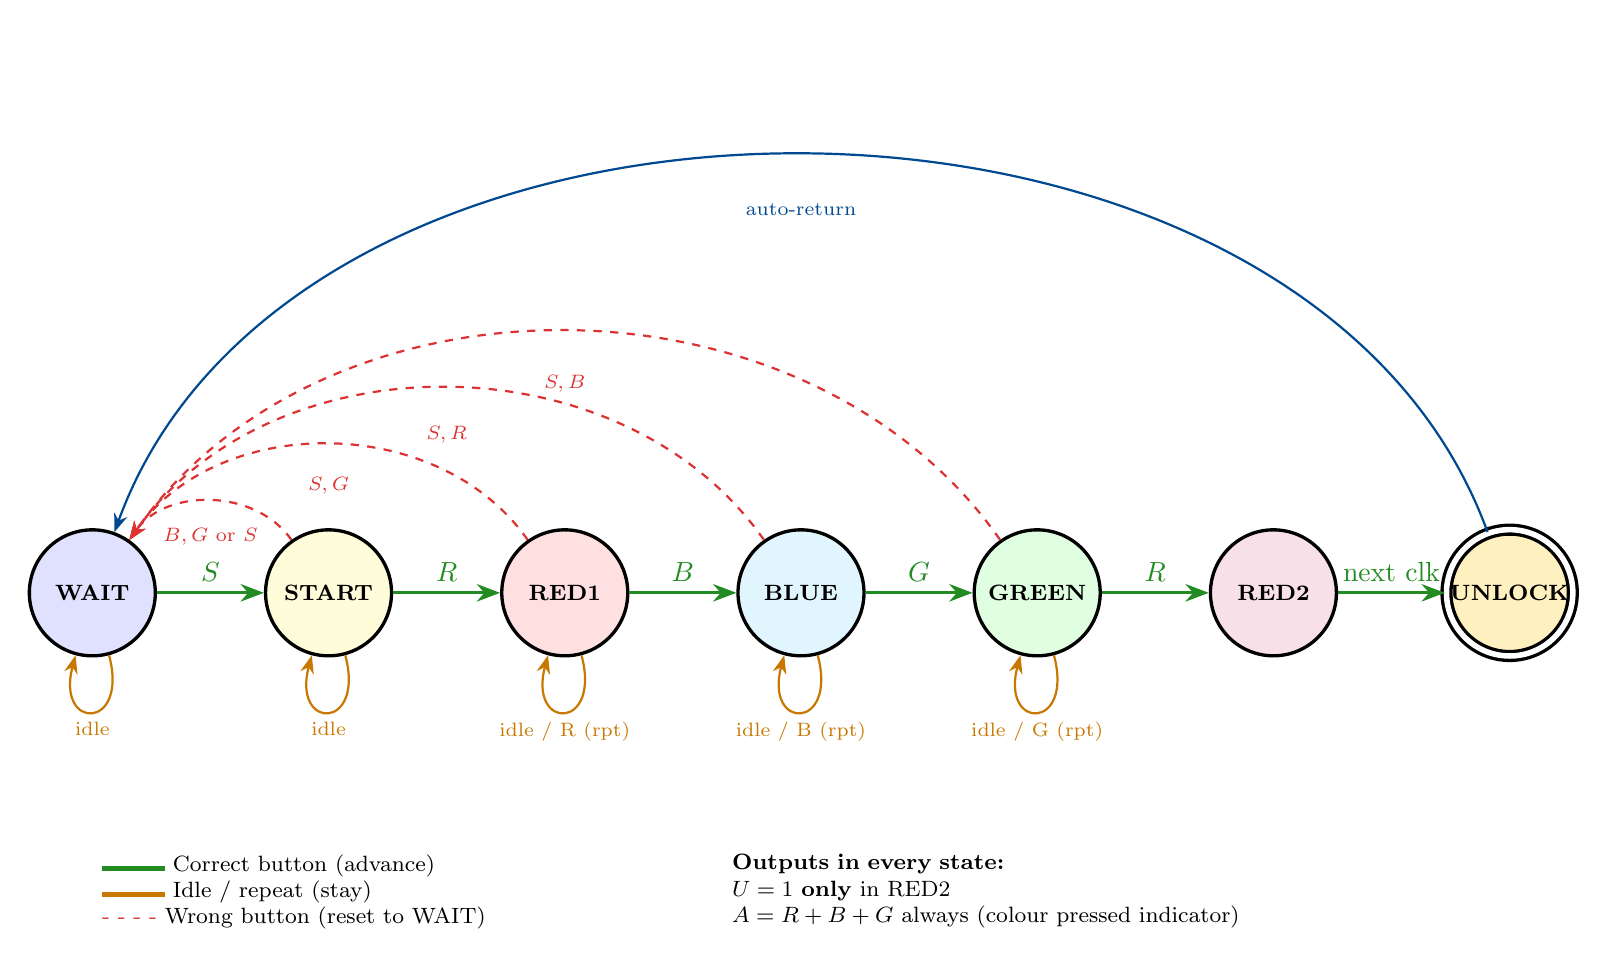
\begin{tikzpicture}[>=Stealth,
  st/.style={circle, draw, very thick, minimum size=1.6cm,
             font=\footnotesize\bfseries, inner sep=1pt},
  every edge/.style={draw, ->, thick, font=\footnotesize},
  node distance=2.8cm
]
  %% ── nodes (linear chain) ──
  \node[st, fill=blue!12]   (W)  at (0,0)   {WAIT};
  \node[st, fill=yellow!15] (S)  at (3,0)   {START};
  \node[st, fill=red!12]    (R1) at (6,0)   {RED1};
  \node[st, fill=cyan!12]   (BL) at (9,0)   {BLUE};
  \node[st, fill=green!12]  (GR) at (12,0)  {GREEN};
  \node[st, fill=purple!12] (R2) at (15,0)  {RED2};
  \node[st, fill=gold!25, double, double distance=2pt]
                             (UL) at (18,0)  {UNLOCK};

  %% ── correct-path arrows (green, above) ──
  \draw[->, successgreen, very thick]
    (W)  -- node[above, text=successgreen]{$S$} (S);
  \draw[->, successgreen, very thick]
    (S)  -- node[above, text=successgreen]{$R$} (R1);
  \draw[->, successgreen, very thick]
    (R1) -- node[above, text=successgreen]{$B$} (BL);
  \draw[->, successgreen, very thick]
    (BL) -- node[above, text=successgreen]{$G$} (GR);
  \draw[->, successgreen, very thick]
    (GR) -- node[above, text=successgreen]{$R$} (R2);
  \draw[->, successgreen, very thick]
    (R2) -- node[above, text=successgreen]{next clk} (UL);

  %% ── self-loops (orange, below each node) ──
  \path (W)  edge[loop below, warncolor, thick, looseness=6]
        node[below, text=warncolor, font=\scriptsize]{idle} (W);
  \path (S)  edge[loop below, warncolor, thick, looseness=6]
        node[below, text=warncolor, font=\scriptsize]{idle} (S);
  \path (R1) edge[loop below, warncolor, thick, looseness=6]
        node[below, text=warncolor, font=\scriptsize]{idle / R (rpt)} (R1);
  \path (BL) edge[loop below, warncolor, thick, looseness=6]
        node[below, text=warncolor, font=\scriptsize]{idle / B (rpt)} (BL);
  \path (GR) edge[loop below, warncolor, thick, looseness=6]
        node[below, text=warncolor, font=\scriptsize]{idle / G (rpt)} (GR);

  %% ── error resets (red dashed, curve underneath) ──
  \draw[->, accent, dashed, thick, bend right=55]
    (S)  to node[below, font=\scriptsize, text=accent, yshift=-6pt]
    {$B,G$ or $S$} (W);
  \draw[->, accent, dashed, thick, bend right=55]
    (R1) to node[below, font=\scriptsize, text=accent, yshift=-8pt]
    {$S,G$} (W);
  \draw[->, accent, dashed, thick, bend right=55]
    (BL) to node[below, font=\scriptsize, text=accent, yshift=-10pt]
    {$S,R$} (W);
  \draw[->, accent, dashed, thick, bend right=55]
    (GR) to node[below, font=\scriptsize, text=accent, yshift=-12pt]
    {$S,B$} (W);

  %% ── return from UNLOCK ──
  \draw[->, primary, thick, bend right=70]
    (UL) to node[below, font=\scriptsize, yshift=-14pt]
    {auto-return} (W);

  %% ── legend ──
  \node[anchor=north west, text width=6cm, font=\footnotesize]
    at (0, -3.2) {
      \textcolor{successgreen}{\rule{0.8cm}{2pt}} Correct button (advance)\\
      \textcolor{warncolor}{\rule{0.8cm}{2pt}} Idle / repeat (stay)\\
      \textcolor{accent}{- - - -} Wrong button (reset to WAIT)
    };

  %% ── output annotations ──
  \node[anchor=north west, text width=7cm, font=\footnotesize]
    at (8, -3.2) {
      \textbf{Outputs in every state:}\\
      $U = 1$ \textbf{only} in RED2\\
      $A = R + B + G$ always (colour pressed indicator)
    };
\end{tikzpicture}
}%
\caption{Sequential Button Lock --- Complete State Diagram}
\label{fig:lock_fsm}
\end{figure}

% ─── 16.5  EDGE CASES ───
\subsubsection{Edge Cases --- Every Scenario Explained}

\begin{table}[H]
\centering
\small
\caption{All Edge-Case Scenarios}
\begin{tabular}{r p{4.8cm} c c c p{3.2cm}}
\toprule
\# & \textbf{Scenario} & \textbf{State} & $U$ & $A$ & \textbf{Next State} \\
\midrule
1 & Press R before S & WAIT & 0 & \textbf{1} & WAIT (ignored) \\
2 & Press B before S & WAIT & 0 & \textbf{1} & WAIT (ignored) \\
3 & Press G before S & WAIT & 0 & \textbf{1} & WAIT (ignored) \\
4 & Press S (correct start) & WAIT & 0 & 0 & START \\
5 & Idle (no button) in START & START & 0 & 0 & START (stay) \\
6 & Press B in START (wrong) & START & 0 & \textbf{1} & WAIT (reset) \\
7 & Press G in START (wrong) & START & 0 & \textbf{1} & WAIT (reset) \\
8 & Press S again in START & START & 0 & 0 & WAIT (reset) \\
9 & Press R in START (correct) & START & 0 & \textbf{1} & RED1 \\
10 & Press R again in RED1 (repeat) & RED1 & 0 & \textbf{1} & RED1 (stay) \\
11 & Press G in RED1 (wrong) & RED1 & 0 & \textbf{1} & WAIT (reset) \\
12 & Press B in RED1 (correct) & RED1 & 0 & \textbf{1} & BLUE \\
13 & Press R in BLUE (wrong) & BLUE & 0 & \textbf{1} & WAIT (reset) \\
14 & Press B in BLUE (repeat) & BLUE & 0 & \textbf{1} & BLUE (stay) \\
15 & Press G in BLUE (correct) & BLUE & 0 & \textbf{1} & GREEN \\
16 & Press B in GREEN (wrong) & GREEN & 0 & \textbf{1} & WAIT (reset) \\
17 & Press G in GREEN (repeat) & GREEN & 0 & \textbf{1} & GREEN (stay) \\
18 & Press R in GREEN (correct) & GREEN & 0 & \textbf{1} & RED2 \\
19 & Arrive in RED2 & RED2 & \textbf{1} & * & UNLOCK \\
20 & Leave UNLOCK (auto) & UNLOCK & 0 & 0 & WAIT \\
21 & S pressed mid-sequence & any & 0 & 0 & WAIT (reset) \\
22 & Idle cycle in any state & any & 0 & 0 & same (stay) \\
23 & Button held 100 clocks & any & -- & \textbf{1} & same (stay) \\
24 & S-R-B-G-B (wrong at end) & GREEN & 0 & \textbf{1} & WAIT (B wrong) \\
25 & Correct seq then immediate S & WAIT & 0 & 0 & START (new attempt) \\
\bottomrule
\end{tabular}
\caption*{\small * $A$ depends on whether a colour button is being pressed at that moment.}
\end{table}

\begin{importantbox}[Key Edge-Case Insights]
\begin{enumerate}
  \item \textbf{$A$ fires even on wrong buttons.} If the user presses Red when Blue was expected, $A$ still goes HIGH because a \emph{colour} was pressed. $A$ is not a ``correct'' indicator --- it is a ``colour-activity'' indicator.
  \item \textbf{$A$ does NOT fire for Start.} $S$ is not a colour, so $A=0$ when only $S$ is pressed.
  \item \textbf{$A$ does NOT fire on idle.} No button $\Rightarrow$ $A=0$.
  \item \textbf{Repeated correct button = stay.} Holding Red in RED1 keeps the FSM in RED1 with $A=1$, waiting for the next distinct press.
  \item \textbf{Wrong colour = instant reset.} Even though $A=1$ lights up, the FSM silently returns to WAIT.
  \item \textbf{$U$ = 1 for exactly one clock.} RED2 $\to$ UNLOCK $\to$ WAIT. The unlock pulse is brief.
\end{enumerate}
\end{importantbox}

% ─── 16.6  STATE ASSIGNMENT ───
\subsubsection{State Assignment (Binary Encoding)}

\begin{table}[H]
\centering
\caption{State Encoding --- 7 states, 3 flip-flops ($Q_2 Q_1 Q_0$)}
\begin{tabular}{l|ccc|l}
\toprule
\textbf{State} & $Q_2$ & $Q_1$ & $Q_0$ & \textbf{Expects Next} \\
\midrule
WAIT    & 0 & 0 & 0 & $S$ (Start) \\
START   & 0 & 0 & 1 & $R$ (Red) \\
RED1    & 0 & 1 & 0 & $B$ (Blue) \\
BLUE    & 0 & 1 & 1 & $G$ (Green) \\
GREEN   & 1 & 0 & 0 & $R$ (Red) \\
RED2    & 1 & 0 & 1 & (done --- unlock) \\
UNLOCK  & 1 & 1 & 0 & (auto $\to$ WAIT) \\
(unused)& 1 & 1 & 1 & $\to$ WAIT (safe) \\
\bottomrule
\end{tabular}
\end{table}

% ─── 16.7  FULL EXCITATION TABLE ───
\subsubsection{Complete Excitation Table}

\begin{table}[H]
\centering
\footnotesize
\caption{Full Excitation Table (D Flip-Flops)}
\begin{tabular}{ccc|cccc|ccc|cc|l}
\toprule
$Q_2$ & $Q_1$ & $Q_0$ & $S$ & $R$ & $B$ & $G$ & $D_2$ & $D_1$ & $D_0$ & $U$ & $A$ & Transition \\
\midrule
\multicolumn{13}{l}{\cellcolor{blue!8}\textbf{WAIT (000)}} \\
0&0&0 & 1&0&0&0 & 0&0&1 & 0&0 & $\to$ START \\
0&0&0 & 0&1&0&0 & 0&0&0 & 0&\textbf{1} & stay (wrong, no S yet) \\
0&0&0 & 0&0&1&0 & 0&0&0 & 0&\textbf{1} & stay \\
0&0&0 & 0&0&0&1 & 0&0&0 & 0&\textbf{1} & stay \\
0&0&0 & 0&0&0&0 & 0&0&0 & 0&0 & stay (idle) \\
\midrule
\multicolumn{13}{l}{\cellcolor{yellow!8}\textbf{START (001) --- expects R}} \\
0&0&1 & 0&1&0&0 & 0&1&0 & 0&\textbf{1} & $\to$ RED1 (correct!) \\
0&0&1 & 0&0&1&0 & 0&0&0 & 0&\textbf{1} & $\to$ WAIT (B wrong) \\
0&0&1 & 0&0&0&1 & 0&0&0 & 0&\textbf{1} & $\to$ WAIT (G wrong) \\
0&0&1 & 1&0&0&0 & 0&0&0 & 0&0 & $\to$ WAIT (S mid-seq) \\
0&0&1 & 0&0&0&0 & 0&0&1 & 0&0 & stay (idle) \\
\midrule
\multicolumn{13}{l}{\cellcolor{red!8}\textbf{RED1 (010) --- expects B}} \\
0&1&0 & 0&0&1&0 & 0&1&1 & 0&\textbf{1} & $\to$ BLUE (correct!) \\
0&1&0 & 0&1&0&0 & 0&1&0 & 0&\textbf{1} & stay RED1 (R repeat) \\
0&1&0 & 0&0&0&1 & 0&0&0 & 0&\textbf{1} & $\to$ WAIT (G wrong) \\
0&1&0 & 1&0&0&0 & 0&0&0 & 0&0 & $\to$ WAIT (S mid-seq) \\
0&1&0 & 0&0&0&0 & 0&1&0 & 0&0 & stay (idle) \\
\midrule
\multicolumn{13}{l}{\cellcolor{cyan!8}\textbf{BLUE (011) --- expects G}} \\
0&1&1 & 0&0&0&1 & 1&0&0 & 0&\textbf{1} & $\to$ GREEN (correct!) \\
0&1&1 & 0&1&0&0 & 0&0&0 & 0&\textbf{1} & $\to$ WAIT (R wrong) \\
0&1&1 & 0&0&1&0 & 0&1&1 & 0&\textbf{1} & stay BLUE (B repeat) \\
0&1&1 & 1&0&0&0 & 0&0&0 & 0&0 & $\to$ WAIT (S mid-seq) \\
0&1&1 & 0&0&0&0 & 0&1&1 & 0&0 & stay (idle) \\
\midrule
\multicolumn{13}{l}{\cellcolor{green!8}\textbf{GREEN (100) --- expects R}} \\
1&0&0 & 0&1&0&0 & 1&0&1 & 0&\textbf{1} & $\to$ RED2 (correct!) \\
1&0&0 & 0&0&1&0 & 0&0&0 & 0&\textbf{1} & $\to$ WAIT (B wrong) \\
1&0&0 & 0&0&0&1 & 1&0&0 & 0&\textbf{1} & stay GREEN (G repeat) \\
1&0&0 & 1&0&0&0 & 0&0&0 & 0&0 & $\to$ WAIT (S mid-seq) \\
1&0&0 & 0&0&0&0 & 1&0&0 & 0&0 & stay (idle) \\
\midrule
\multicolumn{13}{l}{\cellcolor{purple!8}\textbf{RED2 (101) --- UNLOCK}} \\
1&0&1 & X&X&X&X & 1&1&0 & \textbf{1}&* & $\to$ UNLOCK ($U\!=\!1$) \\
\midrule
\multicolumn{13}{l}{\cellcolor{gold!10}\textbf{UNLOCK (110)}} \\
1&1&0 & X&X&X&X & 0&0&0 & 0&* & $\to$ WAIT (auto) \\
\midrule
\multicolumn{13}{l}{\cellcolor{gray!10}\textbf{(UNUSED 111)}} \\
1&1&1 & X&X&X&X & 0&0&0 & 0&0 & $\to$ WAIT (safe) \\
\bottomrule
\end{tabular}
\caption*{\small * $A = R+B+G$ always; shown as \textbf{1} where a colour is pressed.}
\end{table}

% ─── 16.8  BOOLEAN EQUATIONS ───
\subsubsection{Output Equations}

\begin{tipbox}[Final Equations]
\textbf{Unlock output ($U$):} Only HIGH in RED2 ($Q_2 Q_1 Q_0 = 101$):
$$\boxed{U = Q_2 \cdot \overline{Q_1} \cdot Q_0}$$

\textbf{Activity indicator ($A$):} Purely combinational (no state dependence):
$$\boxed{A = R + B + G}$$

This is extremely simple --- just an OR gate on the three colour inputs. It is independent of the FSM state machine entirely.
\end{tipbox}

% ─── 16.9  TIMING DIAGRAM ───
\subsubsection{Timing Diagram --- Correct Sequence}

\begin{figure}[H]
\centering
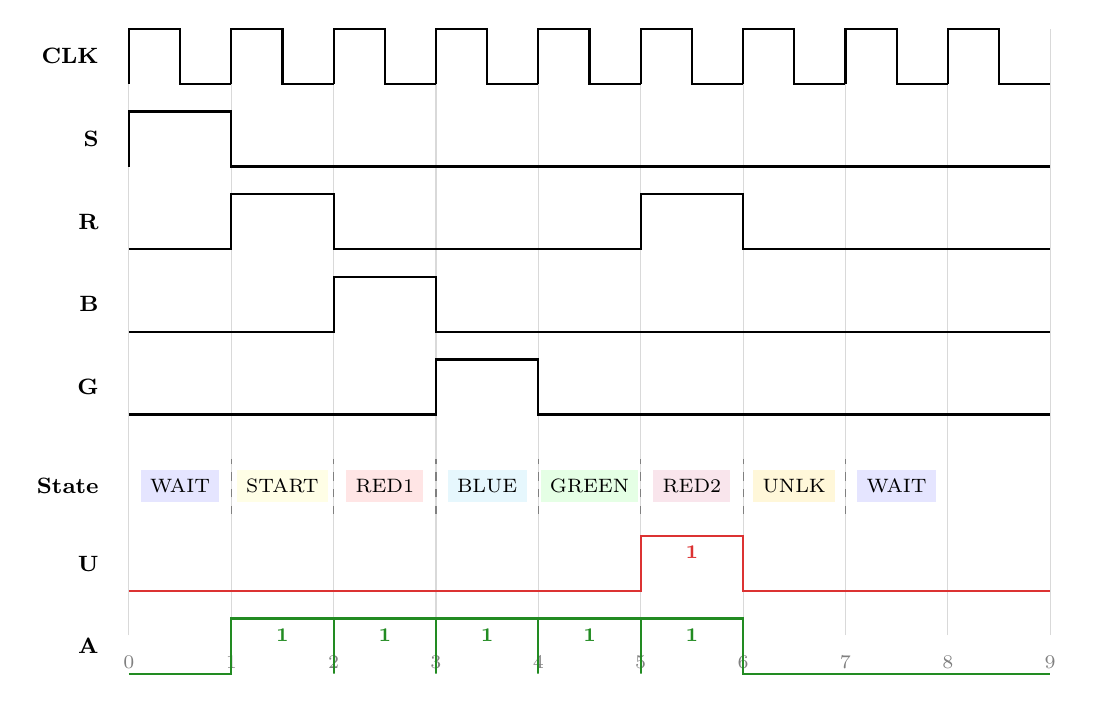
\begin{tikzpicture}[xscale=1.3, yscale=0.7, >=Stealth]
  % Grid
  \foreach \x in {0,1,...,9} {
    \draw[gray!30] (\x, 0) -- (\x, 11);
  }
  \foreach \x in {0,1,...,9} {
    \node[font=\scriptsize, gray] at (\x, -0.5) {\x};
  }

  % Clock
  \node[font=\footnotesize\bfseries, anchor=east] at (-0.2, 10.5) {CLK};
  \foreach \x in {0,1,...,8} {
    \draw[thick] (\x, 10) -- (\x, 11) -- (\x+0.5, 11) -- (\x+0.5, 10) -- (\x+1, 10);
  }

  % S input
  \node[font=\footnotesize\bfseries, anchor=east] at (-0.2, 9) {S};
  \draw[thick] (0,8.5) -- (0,9.5) -- (1,9.5) -- (1,8.5) -- (9,8.5);

  % R input
  \node[font=\footnotesize\bfseries, anchor=east] at (-0.2, 7.5) {R};
  \draw[thick] (0,7) -- (1,7) -- (1,8) -- (2,8) -- (2,7) -- (5,7) -- (5,8) -- (6,8) -- (6,7) -- (9,7);

  % B input
  \node[font=\footnotesize\bfseries, anchor=east] at (-0.2, 6) {B};
  \draw[thick] (0,5.5) -- (2,5.5) -- (2,6.5) -- (3,6.5) -- (3,5.5) -- (9,5.5);

  % G input
  \node[font=\footnotesize\bfseries, anchor=east] at (-0.2, 4.5) {G};
  \draw[thick] (0,4) -- (3,4) -- (3,5) -- (4,5) -- (4,4) -- (9,4);

  % State
  \node[font=\footnotesize\bfseries, anchor=east] at (-0.2, 2.7) {State};
  \node[font=\scriptsize, fill=blue!10] at (0.5, 2.7) {WAIT};
  \node[font=\scriptsize, fill=yellow!10] at (1.5, 2.7) {START};
  \node[font=\scriptsize, fill=red!10] at (2.5, 2.7) {RED1};
  \node[font=\scriptsize, fill=cyan!10] at (3.5, 2.7) {BLUE};
  \node[font=\scriptsize, fill=green!10] at (4.5, 2.7) {GREEN};
  \node[font=\scriptsize, fill=purple!10] at (5.5, 2.7) {RED2};
  \node[font=\scriptsize, fill=gold!15] at (6.5, 2.7) {UNLK};
  \node[font=\scriptsize, fill=blue!10] at (7.5, 2.7) {WAIT};
  \foreach \x in {1,2,3,4,5,6,7} {
    \draw[gray, dashed] (\x, 2.2) -- (\x, 3.2);
  }

  % U output
  \node[font=\footnotesize\bfseries, anchor=east] at (-0.2, 1.3) {U};
  \draw[thick, accent] (0,0.8) -- (5,0.8) -- (5,1.8) -- (6,1.8) -- (6,0.8) -- (9,0.8);
  \node[font=\scriptsize\bfseries, accent] at (5.5, 1.5) {1};

  % A output
  \node[font=\footnotesize\bfseries, anchor=east] at (-0.2, -0.2) {A};
  \draw[thick, successgreen] (0,-0.7) -- (1,-0.7) -- (1,0.3) -- (2,0.3) -- (2,-0.7)
    -- (2,-0.7) -- (2,0.3) -- (3,0.3) -- (3,-0.7)
    -- (3,-0.7) -- (3,0.3) -- (4,0.3) -- (4,-0.7)
    -- (4,-0.7) -- (4,0.3) -- (5,0.3) -- (5,-0.7)
    -- (5,-0.7) -- (5,0.3) -- (6,0.3) -- (6,-0.7)
    -- (9, -0.7);

  % A labels
  \foreach \x in {1.5, 2.5, 3.5, 4.5, 5.5} {
    \node[font=\scriptsize\bfseries, successgreen] at (\x, 0) {1};
  }

\end{tikzpicture}
\caption{Timing Diagram: Correct unlock sequence $S \to R \to B \to G \to R$}
\end{figure}

\subsubsection{Timing Diagram --- Wrong Button Scenario}

\begin{figure}[H]
\centering
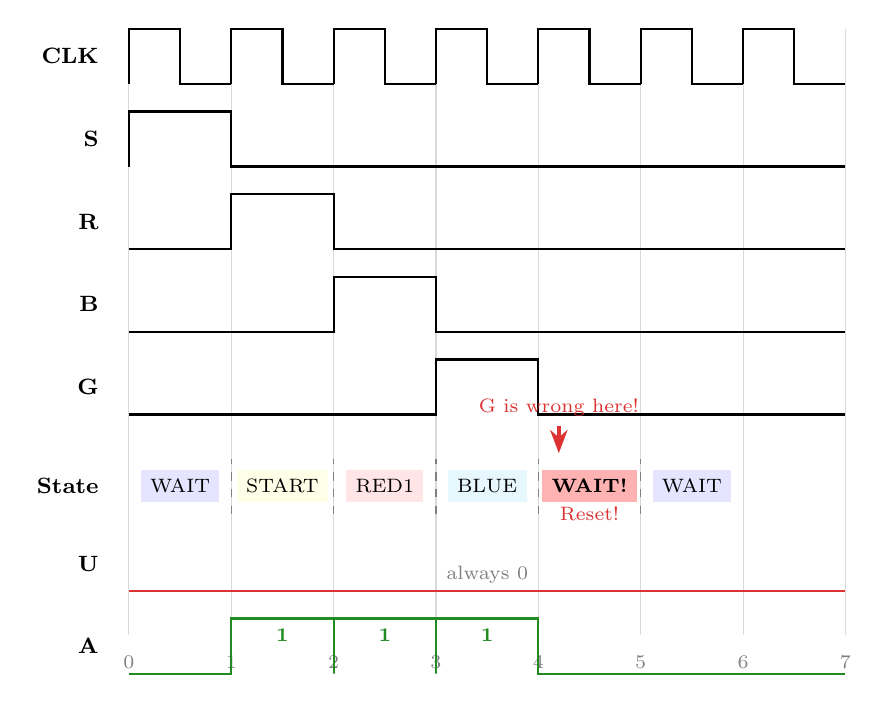
\begin{tikzpicture}[xscale=1.3, yscale=0.7, >=Stealth]
  % Grid
  \foreach \x in {0,1,...,7} {
    \draw[gray!30] (\x, 0) -- (\x, 11);
  }
  \foreach \x in {0,1,...,7} {
    \node[font=\scriptsize, gray] at (\x, -0.5) {\x};
  }

  % Clock
  \node[font=\footnotesize\bfseries, anchor=east] at (-0.2, 10.5) {CLK};
  \foreach \x in {0,1,...,6} {
    \draw[thick] (\x, 10) -- (\x, 11) -- (\x+0.5, 11) -- (\x+0.5, 10) -- (\x+1, 10);
  }

  % S input
  \node[font=\footnotesize\bfseries, anchor=east] at (-0.2, 9) {S};
  \draw[thick] (0,8.5) -- (0,9.5) -- (1,9.5) -- (1,8.5) -- (7,8.5);

  % R input
  \node[font=\footnotesize\bfseries, anchor=east] at (-0.2, 7.5) {R};
  \draw[thick] (0,7) -- (1,7) -- (1,8) -- (2,8) -- (2,7) -- (7,7);

  % B input (wrong --- press at cycle 3 when GREEN expected)
  \node[font=\footnotesize\bfseries, anchor=east] at (-0.2, 6) {B};
  \draw[thick] (0,5.5) -- (2,5.5) -- (2,6.5) -- (3,6.5) -- (3,5.5) -- (7,5.5);

  % G input (pressed where B should have been!)
  \node[font=\footnotesize\bfseries, anchor=east] at (-0.2, 4.5) {G};
  \draw[thick] (0,4) -- (3,4) -- (3,5) -- (4,5) -- (4,4) -- (7,4);

  % State
  \node[font=\footnotesize\bfseries, anchor=east] at (-0.2, 2.7) {State};
  \node[font=\scriptsize, fill=blue!10] at (0.5, 2.7) {WAIT};
  \node[font=\scriptsize, fill=yellow!10] at (1.5, 2.7) {START};
  \node[font=\scriptsize, fill=red!10] at (2.5, 2.7) {RED1};
  \node[font=\scriptsize, fill=cyan!10] at (3.5, 2.7) {BLUE};
  \node[font=\scriptsize, fill=red!30] at (4.5, 2.7) {\textbf{WAIT!}};
  \node[font=\scriptsize, fill=blue!10] at (5.5, 2.7) {WAIT};
  \foreach \x in {1,2,3,4,5} {
    \draw[gray, dashed] (\x, 2.2) -- (\x, 3.2);
  }

  % U output (never goes high)
  \node[font=\footnotesize\bfseries, anchor=east] at (-0.2, 1.3) {U};
  \draw[thick, accent] (0,0.8) -- (7,0.8);
  \node[font=\scriptsize, gray] at (3.5, 1.1) {always 0};

  % A output
  \node[font=\footnotesize\bfseries, anchor=east] at (-0.2, -0.2) {A};
  \draw[thick, successgreen] (0,-0.7) -- (1,-0.7) -- (1,0.3) -- (2,0.3) -- (2,-0.7)
    -- (2,-0.7) -- (2,0.3) -- (3,0.3) -- (3,-0.7)
    -- (3,-0.7) -- (3,0.3) -- (4,0.3) -- (4,-0.7)
    -- (7, -0.7);
  \foreach \x in {1.5, 2.5, 3.5} {
    \node[font=\scriptsize\bfseries, successgreen] at (\x, 0) {1};
  }
  
  % Annotation
  \draw[->, accent, very thick] (4.2, 3.8) -- (4.2, 3.3);
  \node[font=\scriptsize, accent, anchor=south] at (4.2, 3.8) {G is wrong here!};
  \node[font=\scriptsize, accent] at (4.5, 2.2) {Reset!};

\end{tikzpicture}
\caption{Timing Diagram: Wrong button (G pressed when B expected) --- RESET, A still fires}
\end{figure}

% ─── 16.10  STRICT vs LENIENT ───
\subsubsection{Strict vs.\ Lenient Design Comparison}

\begin{table}[H]
\centering
\caption{Design Variations}
\begin{tabular}{p{3cm}|p{4cm}|p{4cm}}
\toprule
\textbf{Scenario} & \textbf{Strict (max security)} & \textbf{Lenient (our design)} \\
\midrule
Same button repeated & $\to$ WAIT (error) & Stay in state \\
$S$ pressed mid-seq & $\to$ WAIT & $\to$ WAIT \\
No timeout & --- & Stay indefinitely \\
$A$ on wrong colour & $A=1$ (same) & $A=1$ (same) \\
$U$ duration & 1 clock & 1 clock \\
\bottomrule
\end{tabular}
\end{table}


% ══════════════════════════════════════════════════════════════════
\section{VHDL Template for FSM Design}
\label{sec:vhdl_template}
% ══════════════════════════════════════════════════════════════════

This section provides a \textbf{universal VHDL template} you can reuse for \emph{any} FSM.  Just change the state names, inputs, outputs, and transition logic.

\subsection{The Three-Process FSM Template}

\begin{infobox}[Three-Process Architecture (Recommended)]
\begin{enumerate}
  \item \textbf{Process 1 --- State Register:} Sequential; updates state on clock edge.
  \item \textbf{Process 2 --- Next-State Logic:} Combinational; computes next state.
  \item \textbf{Process 3 --- Output Logic:} Combinational; computes outputs.
\end{enumerate}
This cleanly separates concerns and is the standard taught in DSD courses.
\end{infobox}

\subsection{Generic VHDL FSM Template}

{\small
\begin{verbatim}
---------------------------------------------------------------
-- GENERIC FSM TEMPLATE (Three-Process Style)
-- Usage: Copy this file, rename entity/architecture,
--        change TYPE state_type, and fill in the CASE blocks.
---------------------------------------------------------------
library IEEE;
use IEEE.STD_LOGIC_1164.ALL;

entity fsm_template is
    Port (
        clk     : in  STD_LOGIC;
        reset   : in  STD_LOGIC;
        -- ===== ADD YOUR INPUTS HERE =====
        input_x : in  STD_LOGIC;
        -- ===== ADD YOUR OUTPUTS HERE =====
        output_y : out STD_LOGIC
    );
end fsm_template;

architecture Behavioral of fsm_template is

    -- ===== STEP 1: DEFINE YOUR STATES =====
    type state_type is (S0, S1, S2, S3);   -- Change these!
    signal current_state, next_state : state_type;

begin

    -------------------------------------------------------
    -- PROCESS 1: STATE REGISTER (Sequential)
    -- This is ALWAYS the same for every FSM.
    -- Just copy it. Never change it.
    -------------------------------------------------------
    STATE_REG: process(clk, reset)
    begin
        if reset = '1' then
            current_state <= S0;            -- Initial state
        elsif rising_edge(clk) then
            current_state <= next_state;
        end if;
    end process STATE_REG;

    -------------------------------------------------------
    -- PROCESS 2: NEXT-STATE LOGIC (Combinational)
    -- This is where YOUR design goes.
    -- For each state, decide next_state based on inputs.
    -------------------------------------------------------
    NEXT_STATE_LOGIC: process(current_state, input_x)
        -- Include ALL inputs in sensitivity list!
    begin
        -- Default: stay in current state (prevents latches!)
        next_state <= current_state;

        case current_state is

            when S0 =>
                if input_x = '1' then
                    next_state <= S1;
                else
                    next_state <= S0;   -- explicit stay
                end if;

            when S1 =>
                if input_x = '1' then
                    next_state <= S2;
                else
                    next_state <= S0;
                end if;

            when S2 =>
                next_state <= S3;       -- unconditional

            when S3 =>
                next_state <= S0;       -- return to start

            when others =>
                next_state <= S0;       -- catch unused states!

        end case;
    end process NEXT_STATE_LOGIC;

    -------------------------------------------------------
    -- PROCESS 3: OUTPUT LOGIC (Combinational)
    --
    -- MOORE: output depends on current_state ONLY
    -- MEALY: output depends on current_state AND inputs
    -------------------------------------------------------

    -- === MOORE VERSION ===
    MOORE_OUTPUT: process(current_state)
    begin
        -- Default outputs (prevents latches!)
        output_y <= '0';

        case current_state is
            when S0 => output_y <= '0';
            when S1 => output_y <= '0';
            when S2 => output_y <= '1';
            when S3 => output_y <= '1';
            when others => output_y <= '0';
        end case;
    end process MOORE_OUTPUT;

    -- === MEALY VERSION (use this OR Moore, not both) ===
    -- MEALY_OUTPUT: process(current_state, input_x)
    -- begin
    --     output_y <= '0';  -- default
    --     case current_state is
    --         when S0 =>
    --             if input_x = '1' then
    --                 output_y <= '1';
    --             end if;
    --         when others =>
    --             output_y <= '0';
    --     end case;
    -- end process MEALY_OUTPUT;

end Behavioral;
\end{verbatim}
}

\subsection{Template Rules --- Never Break These}

\begin{importantbox}[VHDL FSM Rules (Memorise These)]
\begin{enumerate}
  \item \textbf{Sensitivity list must be complete.}
    \begin{itemize}
      \item State register: \texttt{(clk, reset)}
      \item Next-state logic: \texttt{(current\_state, all\_inputs)}
      \item Moore output: \texttt{(current\_state)}
      \item Mealy output: \texttt{(current\_state, all\_inputs)}
    \end{itemize}

  \item \textbf{Always assign default outputs} at the top of every combinational process. This prevents accidental \textbf{latches} (the \#1 FSM bug).

  \item \textbf{Always include \texttt{when others}} in every \texttt{case} statement to handle unused/illegal states.

  \item \textbf{Never use \texttt{rising\_edge}} in a combinational process. Only in the state register process.

  \item \textbf{Never read outputs inside the architecture.} Use internal signals instead.

  \item \textbf{Use enumerated types} (\texttt{type state\_type is (...)}) --- never raw \texttt{STD\_LOGIC\_VECTOR} for states. Let the synthesiser pick the encoding.
\end{enumerate}
\end{importantbox}

\subsection{Applied Template: Button Lock in VHDL}

{\small
\begin{verbatim}
---------------------------------------------------------------
-- Problem 16: Sequential Button Door Lock
---------------------------------------------------------------
library IEEE;
use IEEE.STD_LOGIC_1164.ALL;

entity button_lock is
    Port (
        clk   : in  STD_LOGIC;
        reset : in  STD_LOGIC;
        s     : in  STD_LOGIC;     -- start button
        r     : in  STD_LOGIC;     -- red button
        b     : in  STD_LOGIC;     -- blue button
        g     : in  STD_LOGIC;     -- green button
        u     : out STD_LOGIC;     -- unlock
        a     : out STD_LOGIC      -- activity (colour pressed)
    );
end button_lock;

architecture Behavioral of button_lock is

    type state_type is (WAIT_ST, START_ST, RED1_ST,
                        BLUE_ST, GREEN_ST, RED2_ST,
                        UNLOCK_ST);
    signal current_state, next_state : state_type;

begin

    -- Process 1: State Register
    STATE_REG: process(clk, reset)
    begin
        if reset = '1' then
            current_state <= WAIT_ST;
        elsif rising_edge(clk) then
            current_state <= next_state;
        end if;
    end process STATE_REG;

    -- Process 2: Next-State Logic
    NEXT_STATE_LOGIC: process(current_state, s, r, b, g)
    begin
        next_state <= current_state;   -- default: stay

        case current_state is

            when WAIT_ST =>
                if s = '1' then
                    next_state <= START_ST;
                -- else stay (colour buttons or idle)
                end if;

            when START_ST =>
                if    r = '1' then next_state <= RED1_ST;   -- correct
                elsif b = '1' then next_state <= WAIT_ST;   -- wrong
                elsif g = '1' then next_state <= WAIT_ST;   -- wrong
                elsif s = '1' then next_state <= WAIT_ST;   -- restart
                -- else idle: stay
                end if;

            when RED1_ST =>
                if    b = '1' then next_state <= BLUE_ST;   -- correct
                elsif g = '1' then next_state <= WAIT_ST;   -- wrong
                elsif s = '1' then next_state <= WAIT_ST;   -- restart
                -- r = '1': stay (repeat); idle: stay
                end if;

            when BLUE_ST =>
                if    g = '1' then next_state <= GREEN_ST;  -- correct
                elsif r = '1' then next_state <= WAIT_ST;   -- wrong
                elsif s = '1' then next_state <= WAIT_ST;   -- restart
                -- b = '1': stay (repeat); idle: stay
                end if;

            when GREEN_ST =>
                if    r = '1' then next_state <= RED2_ST;   -- correct
                elsif b = '1' then next_state <= WAIT_ST;   -- wrong
                elsif s = '1' then next_state <= WAIT_ST;   -- restart
                -- g = '1': stay (repeat); idle: stay
                end if;

            when RED2_ST =>
                next_state <= UNLOCK_ST;  -- unconditional

            when UNLOCK_ST =>
                next_state <= WAIT_ST;    -- auto-return

            when others =>
                next_state <= WAIT_ST;    -- safety

        end case;
    end process NEXT_STATE_LOGIC;

    -- Process 3a: Unlock Output (Moore — depends on state only)
    u <= '1' when current_state = RED2_ST else '0';

    -- Process 3b: Activity Output (Mealy — depends on inputs only)
    a <= r or b or g;

end Behavioral;
\end{verbatim}
}

\begin{tipbox}[How to Reuse This Template for Any FSM]
\begin{enumerate}
  \item Copy the generic template.
  \item Change \texttt{state\_type} to list your states.
  \item Change ports to your inputs/outputs.
  \item Fill in the \texttt{case} block in Process 2 with your transitions.
  \item Fill in Process 3 with your output logic.
  \item \textbf{Done.} The state register (Process 1) never changes.
\end{enumerate}
\end{tipbox}


% ══════════════════════════════════════════════════════════════════
\section{Quick Reference: FSM Design Checklist}
% ══════════════════════════════════════════════════════════════════

\begin{tipbox}[Before You Submit Your Design]
\begin{enumerate}[leftmargin=*]
  \item[$\square$] All states have transitions for \emph{all} input combinations
  \item[$\square$] Reset/initial state is clearly defined
  \item[$\square$] No unreachable or dead-end states
  \item[$\square$] Unused state combinations handled (safe state)
  \item[$\square$] State encoding is documented
  \item[$\square$] Excitation table matches state diagram exactly
  \item[$\square$] K-maps are correct (check minterms!)
  \item[$\square$] Boolean equations verified against truth table
  \item[$\square$] Output equations are correct (Moore: state only; Mealy: state + input)
  \item[$\square$] Circuit diagram matches equations
  \item[$\square$] Timing diagram verification attempted
  \item[$\square$] All flip-flops have clock and reset connections
\end{enumerate}
\end{tipbox}


% ══════════════════════════════════════════════════════════════════
\section{Summary of All 16 Problems}
% ══════════════════════════════════════════════════════════════════

\begin{table}[H]
\centering
\footnotesize
\caption{Overview of FSM Design Problems}
\begin{tabular}{clcccc}
\toprule
\# & \textbf{Problem} & \textbf{Level} & \textbf{Type} & \textbf{States} & \textbf{FFs} \\
\midrule
1 & Toggle Switch & Beginner & Moore & 2 & 1 \\
2 & 2-Bit Up Counter & Beginner & Moore & 4 & 2 \\
3 & ``11'' Detector & Beginner & Mealy & 2 & 1 \\
4 & Up/Down Counter & Beg--Int & Moore & 8 & 3 \\
5 & Vending Machine & Intermediate & Moore & 4 & 2 \\
6 & Traffic Light & Intermediate & Moore & 3 & 2 \\
7 & Serial Adder & Intermediate & Mealy & 2 & 1 \\
8 & ``1010'' Detector & Intermediate & Moore & 5 & 3 \\
9 & Elevator Door & Int--Adv & Moore & 4 & 2 \\
10 & SPI Master & Advanced & Moore & 6 & 3 \\
11 & UART Receiver & Advanced & Moore & 5 & 3 \\
12 & Washing Machine & Advanced & Moore & 6 & 3 \\
13 & Combination Lock & Advanced & Mealy & 3 & 2 \\
14 & Memory Controller & Advanced & Moore & 5 & 3 \\
15 & AHB-Lite Bus & Expert & Moore & 5 & 3 \\
16 & Sequential Button Lock & Expert & Mealy & 7 & 3 \\
\bottomrule
\end{tabular}
\end{table}

\vspace{1cm}
\begin{center}
\textit{--- End of FSM Design Guide ---}
\end{center}

\end{document}
